\chapter{ALS-causative FUS mutations impair FUS autoregulation through intron retention}

\label{chapter:fus_meta}

\section{Abstract}

FUS is a ubiquitously expressed multi-domain RNA-binding protein with roles in transcription, splicing and RNA transport. Genetic mutations that cause the fatal neurodegenerative disease Amyotrophic Lateral Sclerosis (Motor Neurone Disease) cluster in the FUS C-terminal nuclear localisation signal (NLS).  These mutations impair the nuclear import of FUS,  shifting localisation to the cytoplasm and the formation of FUS-containing stress granules. However the role of FUS nuclear depletion in disease is still not well understood.  In addition, as FUS protein can bind its own transcript, nuclear loss is expected to alter the level of FUS translation due to impairment of an autoregulatory feedback loop and the exact mechanism of this process has not been fully delineated.

The Fratta lab generated RNA sequencing data from embryonic mouse neuronal tissue where FUS was either knocked out or the NLS removed through mutation. I combined the data with two previously published datasets with similar NLS mutations and FUS knockout mice. To assess differential expression and splicing I employed a joint modelling strategy which boosted the power of detection and increased the confidence in my findings. I found that in both expression and splicing, FUS NLS mutations act as a diminished knockout, with little evidence to support a gain of toxic function in the cytoplasm. When examining FUS itself, I observed that loss of nuclear FUS correlated with the reduction in the splicing of a retained intron transcript, which was validated by RT-PCR. The FUS intron retention transcript is insensitive to nonsense-mediated decay.

My data suggest that disease-associated FUS mutations impair FUS autoregulation which is normally maintained through a retained intron transcript. This work has important implications for both the RNA biology and neurodegenerative disease fields.

\section{Contributions}
\begin{itemize}
	% Check with Pietro
	\item Mice were handled by Dr Cristian Bodo
	\item RNA sequencing libraries were prepared by Dr Nicol Birsa.
	\item RNA was extracted for PCR by Dr Nicol Birsa and Matthew Bentham
	\item RT-PCRs were performed by David Robaldo and Dr Carmelo Milioto
\end{itemize}
All bioinformatic analysis and interpretation was designed and performed by myself in consultation with my supervisors. 
The methods section for RT-PCR was partly written by David Robaldo.


\clearpage
\section{Background}

The most aggressive FUS mutations in ALS are those that completely abolish the nuclear localisation signal (NLS). 
Patients carrying a single copy of the P525L mutation, where the critical proline of the PY motif is mutated \citep{Chio2009}, die around 20 years of age with a disease course of less than 2 years \citep{Shang2016}.
The removal of the NLS mislocalises FUS to the cytoplasm but whether toxicity comes from reducing the nuclear functions of FUS or through a new function in the cytoplasm is still being debated.
In this study I combined RNA-seq data from three different mouse mutants homozygous for a different NLS-ablating mutation and compared them to mice homozygous for FUS knockout alleles. 

\begin{figure}[h!]
	\centering
	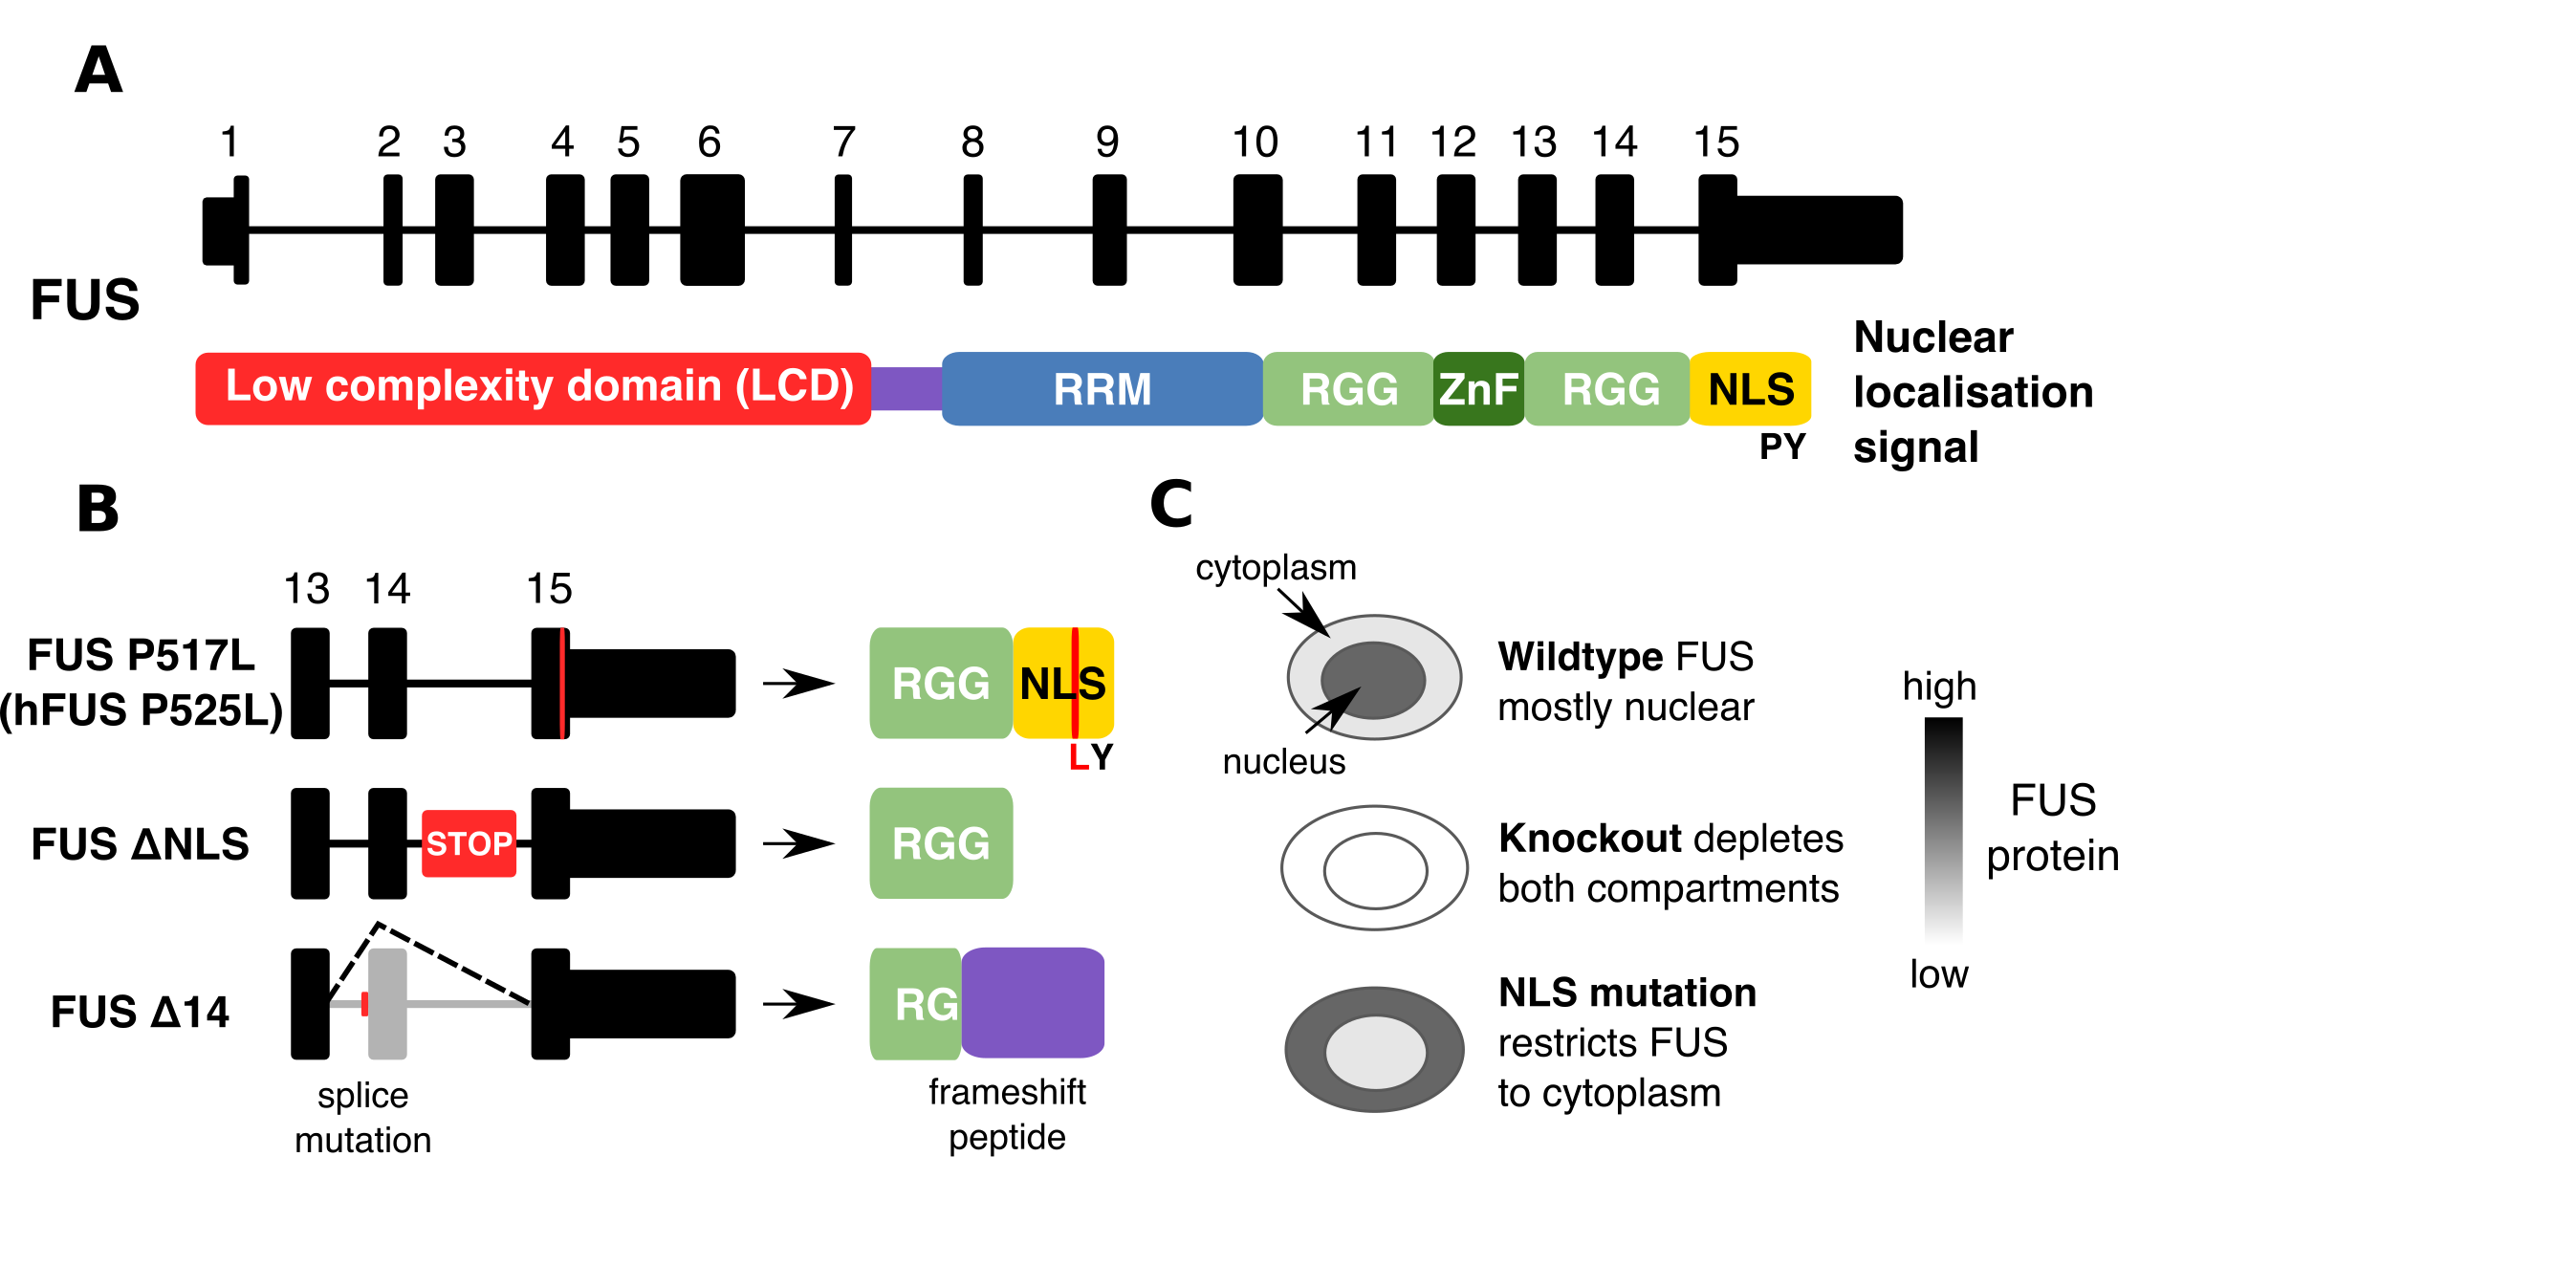
\includegraphics[width=\textwidth]{Figures/06_fus_meta/FUS_structure_mutations.png}
	\caption{\textbf{The structure of the FUS protein and known ALS mutations}}
	A: The FUS protein is comprised of a low complexity domain (LCD), an RNA recognition motif (RRM) domain, two Arginine-Glycine-Glycine (RGG) domains, a zinc finger domain (Znf), a nuclear export signal (NES) and a nuclear localisation signal (NLS). 
	B: The three FUS NLS mutations used in this study. The Bozzoni group knocked in a point mutation to create the FUS P525L line, a missense mutation equivalent to the human ALS P517L mutation.  
	The Dupuis group created a FUS $\Delta$NLS line where the entire NLS is removed.  
	We have used the FUS $\Delta$14 mouse, where a frameshift mutation leads to the skipping of exon 14 and a frameshifting of the remaining NLS sequence.
	C: In wildtype  cells FUS protein is predominantly nuclear but can shuttle to the cytoplasm. When FUS is knocked out it will be reduced in both compartments but if the NLS is mutated or deleted then FUS will accumulate in the cytoplasm.
	
	\label{fig:fus_structure}
\end{figure}


% Discuss 3 datasets, pros and cons of each
% differences in sequencing, prediction
For this study, three datasets of FUS knockout and FUS nuclear localisation signal mutation were used. When combined I refer to them collectively as FUS KO and FUS MUT respectively. Table \ref{tab:fus_datasets} describes the 3 datasets. Table \ref{tab:fus_sequencing} describes the sequencing libraries generated.

\subsubsection{Bozzoni}
Capauto and colleagues from the Bozzoni group generated RNA-seq data from purified motor neurons cultured from mouse induced pluripotent stem cells \citep{Capauto2018}. 
Their knockout uses a gene trap in \textit{Fus} intron 12 first used by Hicks et al \citeyear{Hicks2000}.
This construct leads to a partial reduction of FUS protein levels.
Their NLS mutation is the P525L point mutation \citep{Chio2009}, which in mice corresponds to P517L.  
All mice are homozygous for their transgenes. 
The two conditions share a single set of controls, which are motoneurons derived from wildtype stem cells.
The read depth and length for all the Bozzoni samples is high  and but the sample number is n=3 for each condition, the lowest of the three datasets.
%The sequencing libraries are total RNA rather than polyA enriched which may impact the between-sample variance and make splicing events harder to interpret.
Their differential expression analysis found 40 genes in common, with 198 specific to knockout and 419 specific to NLS mutation. 
Splicing changes were not assessed in their publication.

%Dupuis
\subsubsection{Dupuis}
Scekic-Zahirovic and colleages from the Dupuis group generated RNA-seq data from mouse embryonic brain (embryonic day E18.5) \citep{Scekic-zahirovic2016}. 
Their knockout construct uses a gene trap in \textit{Fus} intron 1 (generated in-house) which leads to complete FUS loss.  
Their NLS mutation introduces a stop codon after exon 14, terminating transcription upstream of the NLS sequence ($\Delta$NLS).  
This mimics the R495X mutation which removes the entire NLS sequence \citep{Bosco2010}.
All mice are homozygous for their transgenes. 
The two conditions have their own separate wildtype littermate controls. 
The depth and read length of the RNA-seq libraries is lower than the other two datasets but this is compensated for by being polyA+ enriched, which will mean a greater proportion of sequencing reads aligning to coding exons.  
%This will be useful for assessing differential expression but I predict the dataset will not be particularly useful for differential splicing due to the low read depth and read length.
They found a strong overlap between differentially expressed genes in the two transgenic lines, with 353 shared genes, 433 specific to FUS NLS mutations and 1205 specific to FUS knockout. 
They also performed a targeted cassette exon splicing analysis (RASL-seq) and again found overlap between knockout and NLS mutation, with 75 shared cassette exons, 98 specific to NLS mutation and 177 specific to knockout. 

% Fratta
\subsubsection{Fratta}
The third dataset was created for this study by the Fratta group from mouse embryonic spinal cord samples (embryonic day E18.5).
 The knockout construct used to generate mice is the same as the Dupuis dataset and hence should be a robust knockout of FUS. 
The NLS mutation is the $\Delta$14 mutation discussed in the previous chapter. A splice acceptor site mutation in exon 14 site prevents exon inclusion, leading to a downstream frameshift and removal of the NLS. 
This mutation corresponds to the human G466VfsX14 mutation \citep{DeJesus-Hernandez2010}.
Each condition, $\Delta$14 and knockout have their own wildtype littermate samples as controls. 
For both conditions, heterozygous mice with only one mutant allele were also generated and sequenced.
The RNA-seq data produced has the longest reads at 2 x 150bp as well as high sequencing depth.
This provides sufficient resolution to quantify differential splicing.\newline

By combining the newly generated Fratta dataset with that of the two previous groups I have put together the largest analysis to date on FUS and gene expression. 
Furthermore I have performed a comprehensive analysis on splicing, looking for both annotated and novel splicing events in both FUS knockout and NLS mutation.
This joint modelling approach boosts statistical power and allows me to demonstrate that the majority of differentially expressed genes and differential splicing events are shared between FUS knockout and NLS mutation.

\clearpage

\begin{longtable}[t]{@{}llllll@{}}
	\begin{minipage}[t]{0.14\columnwidth}\raggedright\strut
		{\textbf{Dataset}}\strut
	\end{minipage} & \begin{minipage}[t]{0.14\columnwidth}\raggedright\strut
		{\textbf{Tissue}}\strut
	\end{minipage} & \begin{minipage}[t]{0.12\columnwidth}\raggedright\strut
		{\textbf{Controls}}\strut
	\end{minipage} & \begin{minipage}[t]{0.10\columnwidth}\raggedright\strut
		{\textbf{Age}}\strut
	\end{minipage} & \begin{minipage}[t]{0.14\columnwidth}\raggedright\strut
		{\textbf{Knockout (KO)}}\strut
	\end{minipage} & \begin{minipage}[t]{0.14\columnwidth}\raggedright\strut
		{\textbf{Mutation (MUT)}}\strut
	\end{minipage}\tabularnewline\toprule \\[-0.3cm] 
	\begin{minipage}[t]{0.16\columnwidth}\raggedright\strut
		{\textbf{Bozzoni}}
		{\footnotesize\citep{Capauto2018}}\strut
	\end{minipage} & \begin{minipage}[t]{0.14\columnwidth}\raggedright\strut
		{Motor neurons}
		{cultured from iPSCs}\strut
	\end{minipage} & \begin{minipage}[t]{0.12\columnwidth}\raggedright\strut
		{Shared}\strut
	\end{minipage} & \begin{minipage}[t]{0.10\columnwidth}\raggedright\strut
		{-}\strut
	\end{minipage} & \begin{minipage}[t]{0.16\columnwidth}\raggedright\strut
		{Gene trap in exon 12}	\strut
	\end{minipage} & \begin{minipage}[t]{0.16\columnwidth}\raggedright\strut
		{P517L knock-in,}
		{corresponding to human P525L}\strut
	\end{minipage}\tabularnewline \\
	\begin{minipage}[t]{0.16\columnwidth}\raggedright\strut
		{\textbf{Dupuis}}
		{\footnotesize\citep{Scekic-zahirovic2016}}\strut
	\end{minipage} & \begin{minipage}[t]{0.14\columnwidth}\raggedright\strut
		{Whole brain}\strut
	\end{minipage} & \begin{minipage}[t]{0.12\columnwidth}\raggedright\strut
		{Separate}\strut
	\end{minipage} & \begin{minipage}[t]{0.10\columnwidth}\raggedright\strut
		{E18.5}\strut
	\end{minipage} & \begin{minipage}[t]{0.16\columnwidth}\raggedright\strut
		{Gene trap in intron 1}\strut
	\end{minipage} & \begin{minipage}[t]{0.16\columnwidth}\raggedright\strut
		{Stop codon after exon 14 ($\Delta$NLS)}\strut
	\end{minipage}\tabularnewline \\
	\begin{minipage}[t]{0.16\columnwidth}\raggedright\strut
		{\textbf{Fratta}}
		{(this study)}\strut
	\end{minipage} & \begin{minipage}[t]{0.14\columnwidth}\raggedright\strut
		{Spinal cord}\strut
	\end{minipage} & \begin{minipage}[t]{0.12\columnwidth}\raggedright\strut
		{Separate}\strut
	\end{minipage} & \begin{minipage}[t]{0.10\columnwidth}\raggedright\strut
		{E18.5}\strut
	\end{minipage} & \begin{minipage}[t]{0.16\columnwidth}\raggedright\strut
		{Gene trap in intron 1}\strut
	\end{minipage} & \begin{minipage}[t]{0.16\columnwidth}\raggedright\strut
		{$\Delta$ exon 14 } \strut
	\end{minipage}\tabularnewline
	\caption{\textbf{The three FUS mouse datasets}}
	\label{tab:fus_datasets}
\end{longtable}

% SEQUENCING STATS

\begin{longtable}[]{@{}llllll@{}}
	\begin{minipage}[t]{0.14\columnwidth}\raggedright\strut
		{\textbf{Dataset}}\strut
	\end{minipage} & \begin{minipage}[t]{0.14\columnwidth}\raggedright\strut
		{\textbf{Replicates per condition}}\strut
	\end{minipage} & \begin{minipage}[t]{0.14\columnwidth}\raggedright\strut
		{\textbf{Library type}}\strut
	\end{minipage} & \begin{minipage}[t]{0.14\columnwidth}\raggedright\strut
		{\textbf{Mapped reads (millions)}}\strut
	\end{minipage} & \begin{minipage}[t]{0.14\columnwidth}\raggedright\strut
		{\textbf{Read type}}\strut
	\end{minipage} & \begin{minipage}[t]{0.14\columnwidth}\raggedright\strut
		{\textbf{SRA accession}}\strut
	\end{minipage}\tabularnewline\toprule \\[-0.3cm]
	\begin{minipage}[t]{0.14\columnwidth}\raggedright\strut
		{\textbf{Bozzoni} }\strut
	\end{minipage} & \begin{minipage}[t]{0.14\columnwidth}\raggedright\strut
		{3}\strut
	\end{minipage} & \begin{minipage}[t]{0.14\columnwidth}\raggedright\strut
		{Total RNA}\strut
	\end{minipage} & \begin{minipage}[t]{0.14\columnwidth}\raggedright\strut
		{34-52}\strut
	\end{minipage} & \begin{minipage}[t]{0.14\columnwidth}\raggedright\strut
		{2 x 100bp}\strut
	\end{minipage} & \begin{minipage}[t]{0.14\columnwidth}\raggedright\strut
		{SRP111475}\strut
	\end{minipage}\tabularnewline \\
	\begin{minipage}[t]{0.14\columnwidth}\raggedright\strut
		{\textbf{Dupuis}}\strut
	\end{minipage} & \begin{minipage}[t]{0.14\columnwidth}\raggedright\strut
		{4-5}\strut
	\end{minipage} & \begin{minipage}[t]{0.14\columnwidth}\raggedright\strut
		{mRNA}\strut
	\end{minipage} & \begin{minipage}[t]{0.14\columnwidth}\raggedright\strut
		{15-25}\strut
	\end{minipage} & \begin{minipage}[t]{0.14\columnwidth}\raggedright\strut
		{1 x 50bp}\strut
	\end{minipage} & \begin{minipage}[t]{0.14\columnwidth}\raggedright\strut
		{SRP070906 }\strut
	\end{minipage}\tabularnewline \\
	\begin{minipage}[t]{0.14\columnwidth}\raggedright\strut
		{\textbf{Fratta} }\strut
	\end{minipage} & \begin{minipage}[t]{0.14\columnwidth}\raggedright\strut
		{4}\strut
	\end{minipage} & \begin{minipage}[t]{0.14\columnwidth}\raggedright\strut
		{Total RNA}\strut
	\end{minipage} & \begin{minipage}[t]{0.14\columnwidth}\raggedright\strut
		{52-65}\strut
	\end{minipage} & \begin{minipage}[t]{0.14\columnwidth}\raggedright\strut
		{2 x 150bp}\strut
	\end{minipage} & \begin{minipage}[t]{0.14\columnwidth}\raggedright\strut
		{-}\strut
	\end{minipage}\tabularnewline
	\caption{\textbf{RNA-seq statistics of the three datasets}}
	\label{tab:fus_sequencing}
\end{longtable}

\clearpage

\section{Methods}

\subsection{RNA sequencing}

All mice used were sacrificed at embryonic day 18.5.
Mice carrying one or two copies of each the FUS knockout transgene from \citep{Scekic-zahirovic2016} or the FUS $\Delta14$ genotype from \citep{Devoy2017} were compared to their wildtype littermates.
Total RNA was extracted from mouse spinal cord. cDNA libraries were created using a TruSeq stranded total RNA RiboZero protocol (Illumina). 
Libraries were sequenced on an Illumina HiSeq to generate paired end 150bp reads. 


\subsection{Data processing}
All RNA sequencing data was processed with our in-house pipeline (outlined in Methods chapter).

\subsection{Differential Expression}
 Each dataset consists of FUS knockout samples, FUS NLS mutation samples and wildtype controls.
In the Bozzoni dataset the controls are shared but in the other two datasets the knockout and mutation samples have their own separate controls for use in two-way comparisons.
Differential gene expression was tested with DESeq2 \citep{Love2014}.
Initially each comparison (wildtype vs knockout or wildtype vs mutation) was performed separately for each dataset, creating six individual analyses.
To boost power and create a set of high confidence changes, two joint models were created using either the knockout (KO) or mutation (MUT) samples with their specific controls.
The joint model uses all the samples of the same comparison together in a general linear model with a dataset covariate. 
DESeq2 uses a Bayesian shrinkage strategy when estimating the $log_2$ fold change. 
%Due to high inter-dataset variability this results in very small fold changes being called.
For each gene the $log_2$ fold change is the linear combination of the three individual datasets.
Genes are reported as significantly differentially expressed at a false discovery rate (FDR) threshold of 0.05 \citep{Benjamini1995}. 
For plots, gene expression values are  raw counts multiplied by each sample's size factor generated by DESeq2. 
These normalised counts are then normalised to the wildtype samples for each dataset to visualise the relative change in expression.

To assess the level of overlap between the KO and MUT joint models, two different overlap thresholds were employed.
The first, a more conservative threshold, depends on a gene being significant at FDR < 0.05 in both datasets.
The second, more relaxed threshold, calls a gene as significant if it falls below FDR < 0.05 in one dataset and has an uncorrected P-value < 0.05 in the other.

\subsection{Differential Splicing}
SGSeq was run on all the samples together to discover and classify all potential splicing events using the default parameters for finding novel splicing \citep{Goldstein2016}. 
Differential splicing for individual comparisons and joint models with a dataset-specific covariate were performed using DEXSeq \citep{Anders2012}.
The same overlap threshold strategies were employed as for differential gene expression.
SGSeq looks for all potential splicing events in each sample and then counts the reads supporting either the inclusion or exclusion of that splicing variant. 
Percentage Spliced In (PSI) values  \citep{Katz2010-ir} for each splicing variant were calculated by taking the read counts supporting the inclusion event and dividing by the total reads in that event. 
% will I bother doing this?
%For individual splicing events, PSI values were compared between each condition using a one-way ANOVA with post-hoc Tukey test.

\subsection{Gene Ontology}
Gene Ontology enrichment testing was performed with the GProfileR package \citep{Reimand2016}. 
GO and KEGG categories were hand-curated to remove redundant terms and restricted to a minimum overlap of 5 genes per set. 
All P-values  are reported after Bonferroni correction. 

\subsection{iCLIP and functional analyses}

FUS iCLIP data from mouse brain \citep{Rogelj2012} was reprocessed by the iCOUNT iCLIP analysis pipeline (http://icount.biolab.si/). 
I downloaded the set of FUS iCLIP clusters that passed enrichment against background at FDR < 0.05. 
Only iCLIP clusters with a minimum of two supporting reads were used. 
Untranslated region (UTR) and coding exon (CDS) annotation were taken from GENCODE mouse (comprehensive; mouse v12). Any intron-retention, nonsense mediated decay or "cds end nf" transcripts were removed. 
UTR coordinates were split into 5' and 3' UTR based on whether they overlapped an annotated polyadenylation site or signal (GENCODE mouse v18 poladenylation annotation). 
3'UTRs were extended by 5kb downstream to capture any unannotated sequence.
Introns were defined as any gaps in the transcript model between CDS and UTR coordinates.
Promoter-antisense coordinates were taken by flanking the 5'UTR sequence by 5kb upstream and inverting the strand.
Overlaps between iCLIP clusters and genomic features were created for each set of differentially expressed genes, split into upregulated ($log_2$ fold change > 0) or downregulated ($log_2$ fold change < 0). 
Overlaps were done in a strand-specific manner, with only iCLIP clusters in the same direction being used.
The difference in proportions of upregulated and downregulated genes for each feature were tested with the $\chi^2$ test of equal proportions.

% functional enrichment tests
For the splicing events found in the joint models, three enrichment tests were performed for different genomic features. 
For these tests the coordinates of the entire encompassing intron were used for each splicing variant.
For a null set of splicing events for comparison, a randomly chosen set of 1000 splicing events of each type were used.
Proportions of overlap between splicing events and the null expectation were tested using a $\chi^2$ test of equal proportions.

The coordinates of polyadenylation cleavage sites were downloaded from the PolyA Site Atlas \citep{Gruber2016}. 
The proportions of  splicing events that overlapped a polyadenylation cleavage site were compared to the null.

The proportion of events of each variant type that overlapped at least one iCLIP peak  were compared to the null expectation.

Per nucleotide PhyloP conservation scores \citep{Pollard2010-fj} comparing mouse (mm10) with 60 other vertebrates was downloaded from UCSC. 
The median PhyloP score was calculated for each splicing variant and compared.

\subsection{RT-PCR}
Primers were designed using Primer3 \citep{Koressaar2007} and in silico PCR (UCSC). 
For both human and mouse FUS, the forward primer was designed for exon 6 and the reverse primer designed to span the spliced exon 8/9 junction to preferentially amplify spliced FUS mRNA. 
An additional third primer was designed to amplify a section of either intron 6 or intron 7.

Cells were obtained from mouse spinal cord and/or cultured mouse embryonic fibroblasts resuspended in Trizol (Thermo Fisher). 
RNA was extracted using miRNeasy Mini Kit (Qiagen) following the manufacturer's instructions % what kit did Nicol use?
cDNA was obtained from extracted RNA using SuperScript IV Reverse Transcriptase kit (Thermo Fisher). 
Briefly, a mix was made of RNA template (500ng for mouse brain; 100ng for cultured cells (cycloheximide treatment), 10 mM dNTP, 50 mM oligo d(T)20, 50 mM random hexamer followed by 5 min of incubation at 65$\degree$C and 1 min in ice. Mix was then complemented with 5X SuperScript IV Reverse Transcriptase buffer, 100 nM DTT, RNase OUT and SuperScript IV Reverse Transcriptase buffer followed by incubation at 23$\degree$C, 55$\degree$C and 80$\degree$C, 10 min each. 

RT-PCR was carried out using 10X AccuPrime Taq DNA polymerase mastermix system (Invitrogen). 
Each PCR reaction mix contained 5 ng of gDNA, 10 mM of forward and reverse primers. cDNA was amplified with the following conditions:
Intron 6 retention: One cycle of 5 min at 95$\degree$C, followed by 30 cycles of 30 sec at 95$\degree$C, 30 sec at 56$\degree$C, and 30 sec at 68$\degree$C, and finishing with 5 min incubation at 68$\degree$C.
Intron 7 retention: One cycle of 5 min at 95$\degree$C, followed by 30 cycles of 30 sec at 95$\degree$C, 30 sec at 61$\degree$C, and 30 sec at 68$\degree$C, and finishing with 5 min incubation at 68$\degree$C.
Srsf7 NMD positive control: One cycle of 5 min at 95 $\degree$C, followed by 35 cycles of 30 sec at 95 $\degree$C, 30 sec at 58 $\degree$C, and 15 sec at 68 $\degree$C, and finishing with 5 min incubation at 68 $\degree$C.
Amplified products were finally obtained using Agilent 4200 TapeStation System following the manufacturer's instructions. Results were analysed on TapeStation analysis software (Agilent).
Intron retention events are plotted  as the percentage of integrated area of band corresponding to intron retention.



\begin{table}[h!]
	%\begin{centerline}
	\centering
	\begin{tabular}{rcl}
		\textbf{Target} & \textbf{Direction} & \textbf{Sequence}\\
		\hline \\[-0.3cm]
		mFUS exon 6  & F &  GTTATGGCAATCAGGACCAGAG\\
		mFUS intron 6 & R & TTGGCTCCCAAGTTCTCACA\\
		mFUS intron 7 & F &  GGAGAAACTGGATGGATGCAC\\
		mFUS exon 8/9 & R &  CCTGTTCAGAATCATGACGAGA\\[0.2cm]
		hFUS exon 6 & F & TCCTCCATGAGTAGTGGTGGT \\
		hFUS intron 6 & R & GTTCAGGCTCCCAAGTTCTC\\
		hFUS intron 7 & F & TTCTCTCGGGTGAGAGAACC\\
		hFUS exon 8/9 & R & GTCTGAATTATCCTGTTCGGAGTC\\[0.2cm]
		mSRSF7 & F &  CGACGAAGAAGAAGCAGGTTTC\\
		mSRSF7& R & TCTGGCCTCTTATGCTGATCAC\\
	\end{tabular}
	%\end{centerline}
	\caption{\textbf{List of primers used in RT-PCR. mFUS: mouse \textit{FUS}; hFUS: human \textit{FUS}}}
	\label{tab:fus_primers}
\end{table}

\subsection{Cycloheximide treatment and fractionation}
Mouse embryonic fibroblasts were treated with 100ug/ml cycloheximide (Sigma) for 6 hours before RNA was extracted with Trizol (Thermo Fisher) and RT-PCR performed as before. 
As a positive control, primers targeting the NMD-sensitive exon 4 of \textit{Srsf7} were used from \citep{Edwards2016}.

\clearpage


\section{Results}

\subsection{Modelling differential expression jointly increases power and demonstrates significant overlap between FUS knockout and FUS NLS mutation}

% Explain individual analyses
Differential expression compares the abundances of transcripts from each gene between two conditions. 
As most RNA-sequencing datasets comprise small numbers of samples, the number of genes found to be significantly changed between conditions depends on the degree of difference between conditions, the number of samples per condition, and the read depth covering each gene. 
%The more sequencing reads that cover a gene, the more precise the measure of the true variance can be.
%Most software packages borrow information across all genes to shrink the variance between samples of the same condition. 
When I analyse each dataset individually, comparing knockout and NLS mutation to their respective controls in each dataset, the Dupuis dataset had the largest number of differentially expressed genes in both conditions (FDR < 0.05), an order of magnitude more than Bozzoni or Fratta (Table \ref{tab:expression_results}). 
Despite the differences in numbers, in all three datasets the knockout condition produces more differentially expressed genes than NLS mutation, suggesting a larger effect on FUS function.

% TABLE OF GENE EXPRESSION NUMBERS
\begingroup
\renewcommand{\arraystretch}{1.5}
\begin{table}[h!]
	%\begin{centerline}
	\begin{tabular}{|r|ccc|ccc|}
		\hline
		& Bozzoni & Dupuis & Fratta & Bozzoni & Dupuis & Fratta\\[-0.3cm]
		& MUT & MUT & MUT & KO & KO & KO\\
		\hline
		Individual hits                & 19 & 1552 & 88 & 100 & 2916 & 151 \\
		Overlapping joint model & 5 & 368 & 57 & 51 & 1007 & 114 \\
		Unique to dataset          & 14 & 1184 & 31 & 49 & 1909 & 37 \\
		\hline
		\textbf{Joint model}       & \multicolumn{3}{c|}{754} & \multicolumn{3}{c|}{2136} \\
		\hline
		Overlap (strict)              & \multicolumn{2}{c}{329} & \multicolumn{2}{|c|}{\textbf{425}} & \multicolumn{2}{c|}{1711} \\
		Overlap (relaxed)           & \multicolumn{2}{c}{186} & \multicolumn{2}{|c|}{\textbf{1318} } & \multicolumn{2}{c|}{961} \\
		\hline
	\end{tabular}
	%\end{centerline}
	\caption{\textbf{Results from separate and joint differential expression analysis}}
	\label{tab:expression_results}
\end{table}
\endgroup


% Combining datasets in a joint model increases power, shrinks effect sizes
I then combined the three datasets together in a joint analysis for the knockout and NLS mutation samples and their respective controls. 
I will refer to these two joint models as KO and MUT respectively.
This increases the sample size of each condition from 3-5 to 11-12 which should markedly improve the estimation of per-gene variation. 
DESeq2 uses a general linear model framework so I  added a dataset-specific covariate. 
This strategy will reward genes where the direction of change is the same between all three datasets and punish genes where the datasets differ in direction. 
The two comparisons are nominally independent from each other as only the Bozzoni wildtype samples are shared.
Modelling all the data together allows the three independent studies of FUS function to contribute to a high-confidence set of expression changes. 
At FDR < 0.05 the KO joint model contains 2136 significantly changed genes and the MUT model contains 754. 
When comparing the genes found by the joint analysis to the individual analyses there is only a moderate overlap. 
Of the 2916 genes found in the Dupuis knockuts, only 1007 of those genes are present in the joint KO analysis.
This suggests that a large number of genes called as significant in each dataset cannot be replicated in the other two datasets, despite being the same condition and all being embryonic neuronal tissue.

\begin{figure}[ht!]
	\centering
	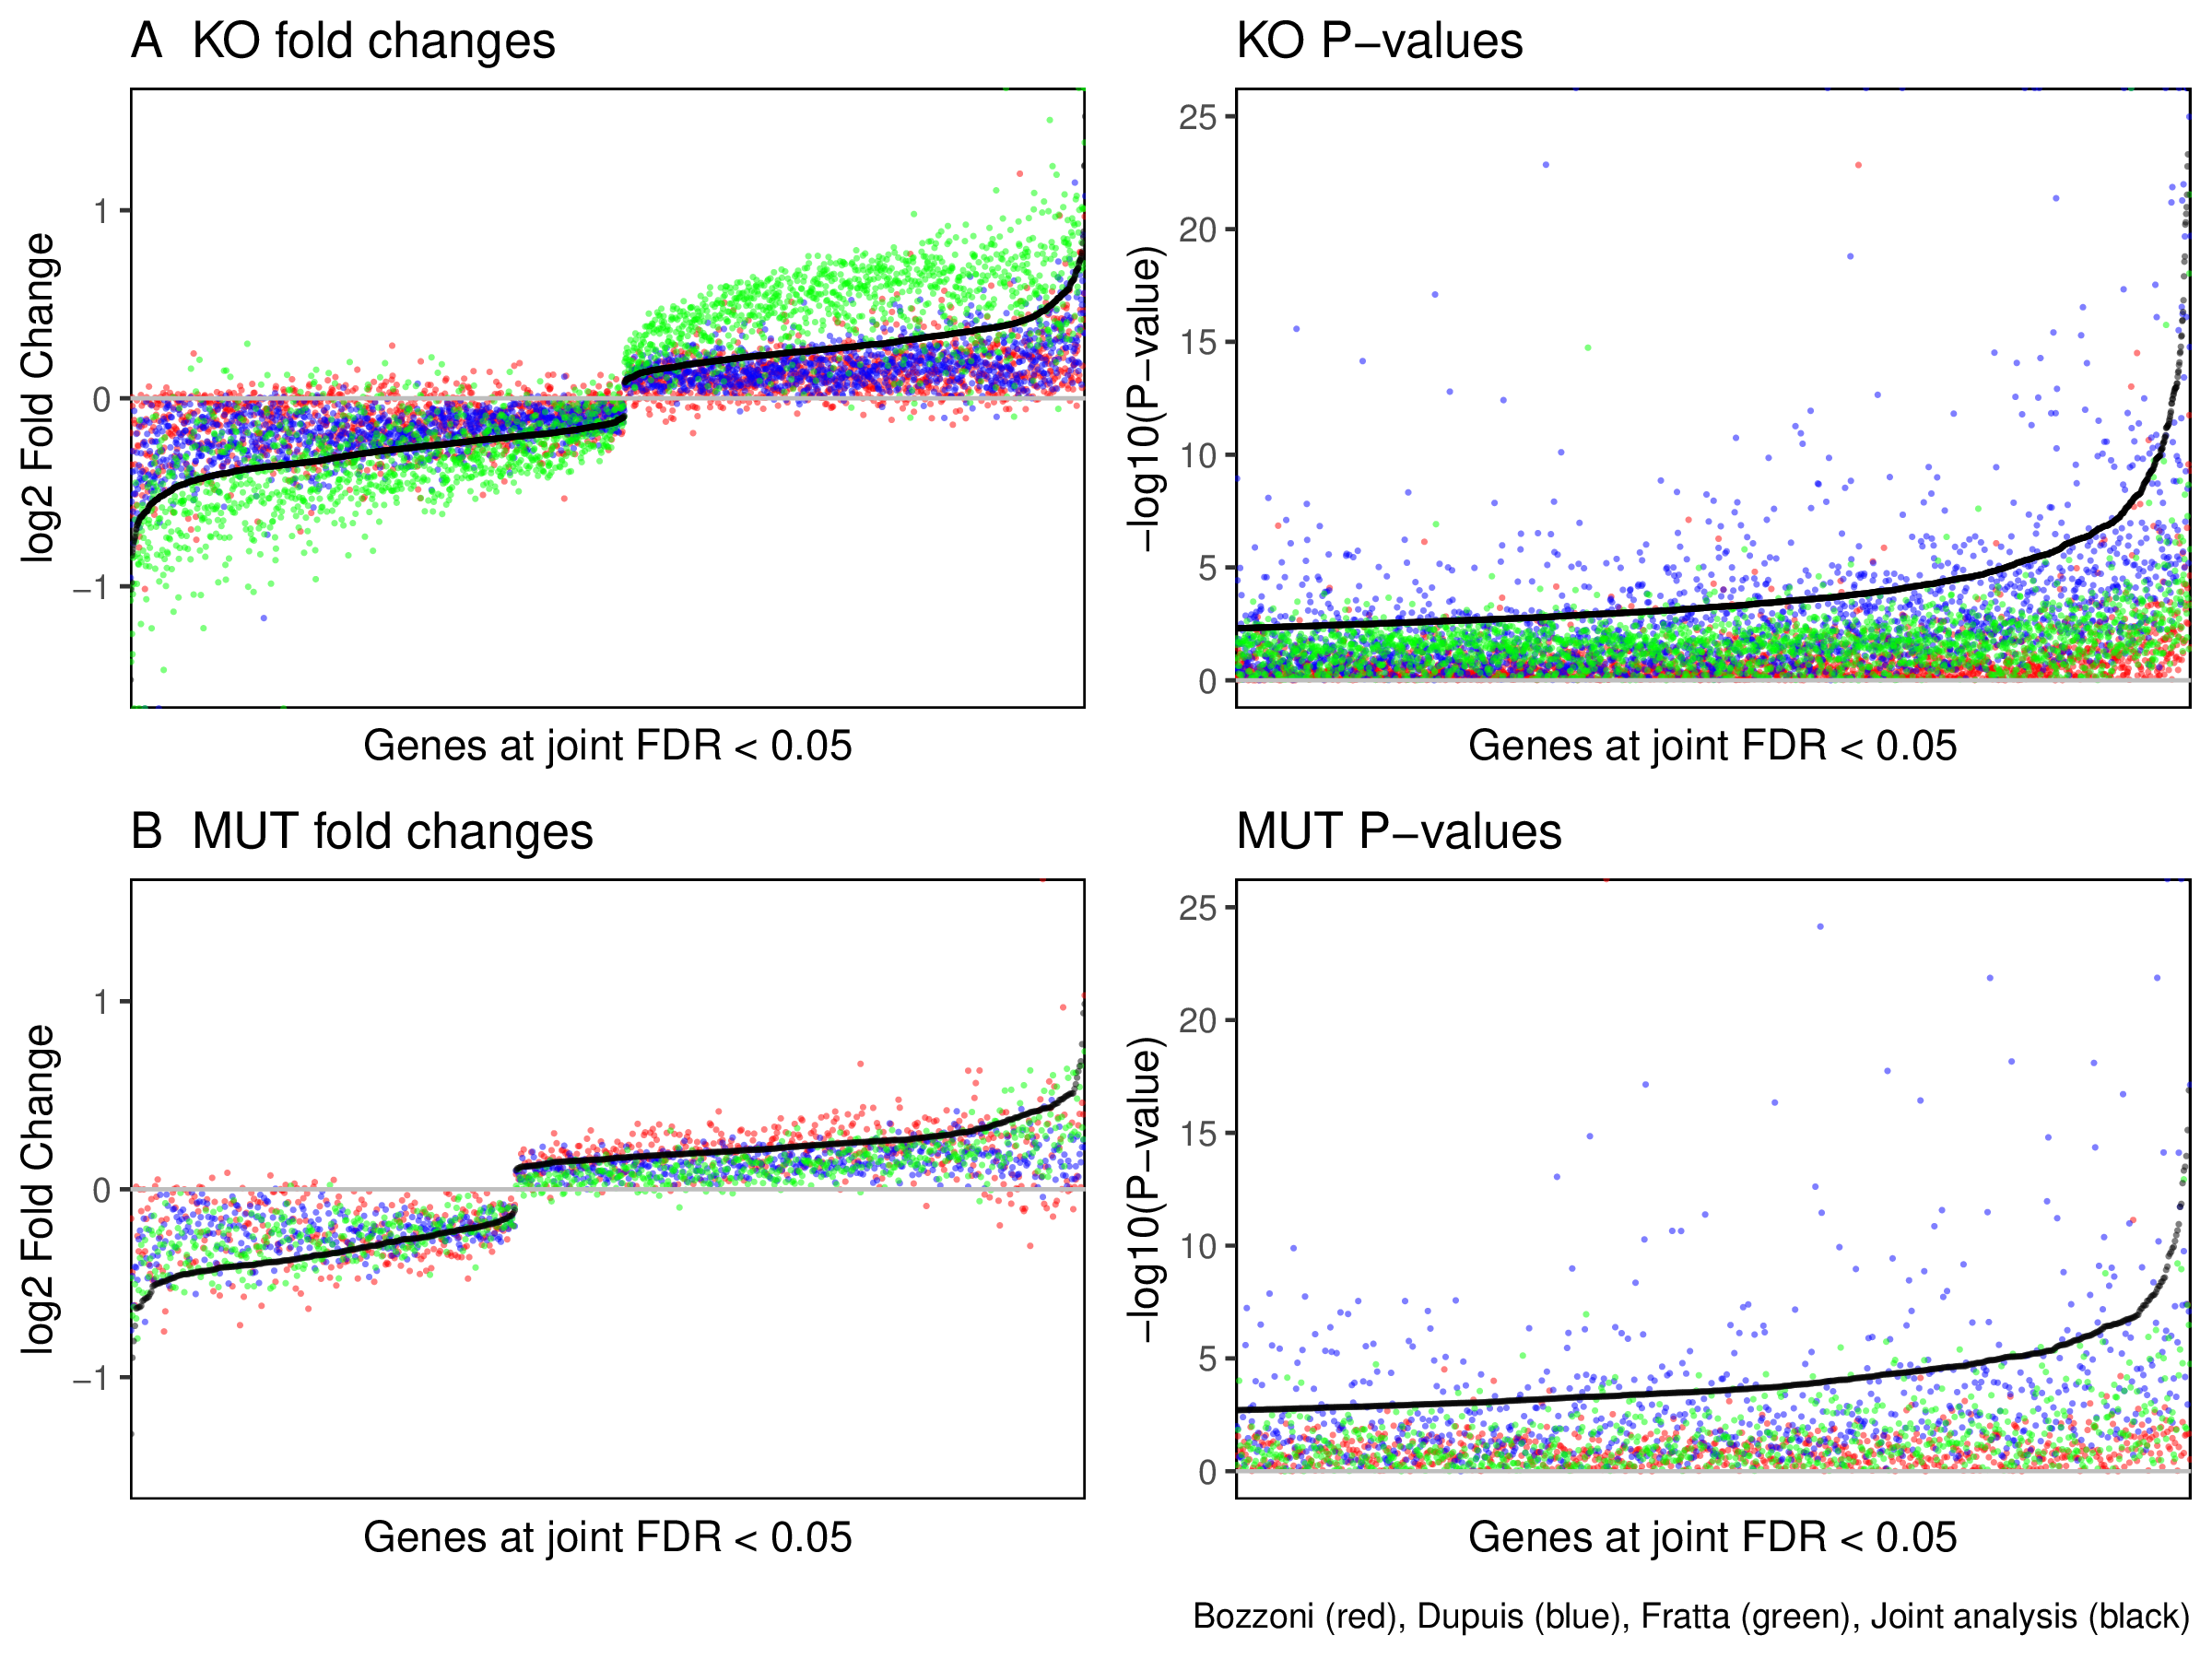
\includegraphics[width=\textwidth]{Figures/06_fus_meta/fitted_vs_individual_p_lfc.png}
	\caption{\textbf{Joint differential expression increases power and adjusts effect sizes}}
	A: Plotting the $log_2$ fold changes (left) and P-values (right) for the 2136 KO genes and 754 MUT genes found at FDR < 0.05 in the two joint analyses. Values found in the individual analyses, Bozzoni (red), Dupuis(blue) and Fratta (green) are compared to the value produced by the joint analysis (black).
	B: As before but for the MUT analyses.
	\label{fig:value_comparison}
\end{figure}

For each gene the resulting joint $log_2$ fold change and P-value is an estimated combination of the three datasets.
I compared the values found by the individual analyses with the joint models(Fig. \ref{fig:value_comparison}).
For the KO models, the Fratta knockout comparison has larger $log_2$ fold change values for the same genes when compared to Bozzoni and Dupuis knockouts. 
The fitted $log_2$ fold change is a compromise between the estimated fold changes of all three datasets. 
When inspecting the distribution of P-values, the Dupuis KO dataset has a excess of low P-values compared to the other two.
Therefore the joint modelling strategy increases the number of genes and harmonises three different datasets together into a set of high confidence differentially expressed genes.

% Explain strict and relaxed overlap

\begin{figure}[ht!]
	\centering
	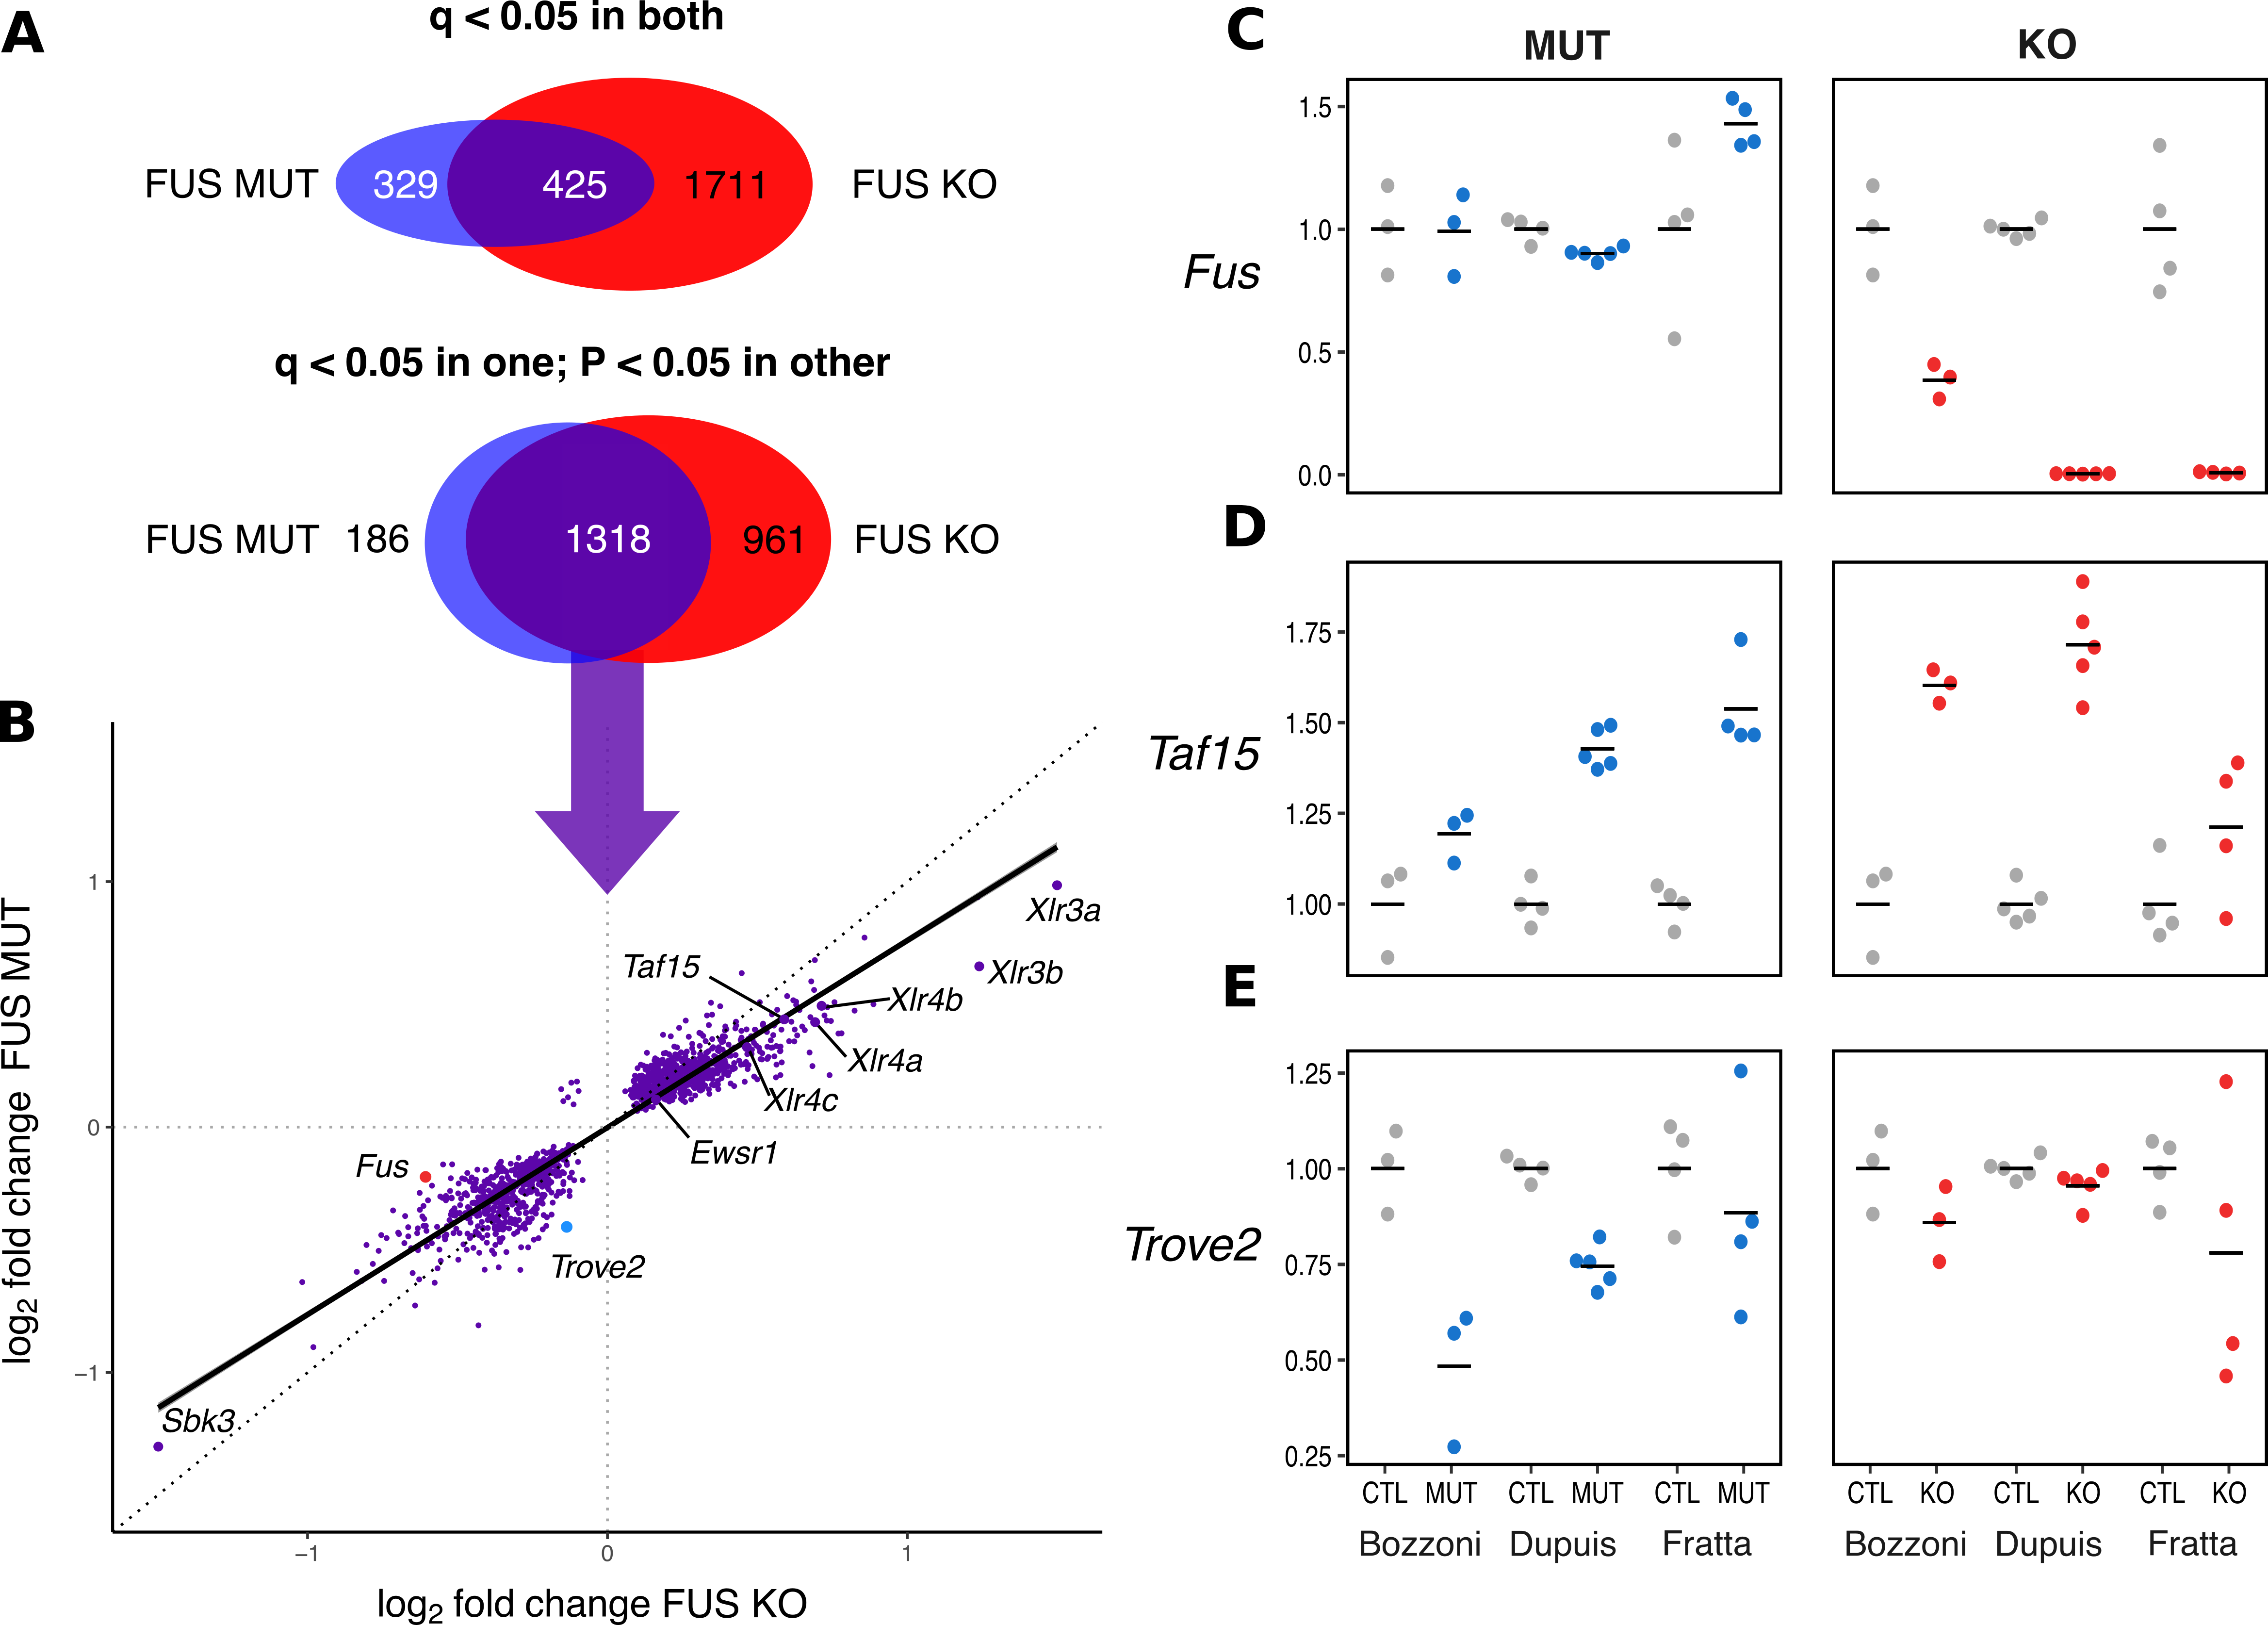
\includegraphics[width=\textwidth]{Figures/06_fus_meta/expression_multi.png}
	\caption{\textbf{Overlapping the joint differential expression models shows that FUS mutations affect gene expression in generally the same direction}}
	A: Venn diagrams show the overlap between the FUS KO and FUS MUT joint differential expression models with a strict FDR cut-off (upper) and a more relaxed P-value cut-off. 
	B: Plotting the fitted $log_2$ fold-change values for each of the 1318 overlapping genes in KO and MUT shows a bias towards weaker changes in MUT compared to KO.
	C, D,E: Normalised read counts in each dataset for \textit{Fus}, \textit{Taf15} and \textit{Trove2}. Samples are plotted relative to the mean expression in controls (CTL).
	\label{fig:fus_expression_multipanel}
\end{figure}

The joint models provide two set of genes where we can be confident of a shared signal between the three datasets.  
I next looked for evidence of a shared gene expression signal between the KO model and the MUT model.
%If there truly is a cytoplasmic gain of FUS function on gene expression then I would expect to see a set of genes specific to NLS mutation or a set of overlapping genes that change in opposing directions.
I first used a conservative threshold for overlap, where a gene must be significant at FDR < 0.05 in both models. 
This produced an overlap of 425 shared genes between KO and MUT (Fig. \ref{fig:fus_expression_multipanel}A), with 329 mutation-specific genes and 1711 knockout specific genes.
I next used  a relaxed overlap criteria where a gene overlaps if it reaches FDR < 0.05 in one model and an uncorrected P < 0.05 in the other.
This increased the overlap to 1318 genes, reducing the specific genes to 186 in the MUT model, and 961 in KO.
The majority of genes are now shared between the two models.

% comparing directions in the overlapping genes
Comparing the log$_2$ fold changes found for the 1318 overlapping genes between FUS KO and FUS MUT showed that only 7 genes are altered in opposing directions (Fig. \ref{fig:fus_expression_multipanel}B) .
Fitting a linear model between the fold changes of the two datasets shows that the effect of FUS MUT on gene expression is 76\% that of FUS KO.  ($\beta$ = 0.76; P < 1e-16 F-test; $R^2$ = 0.90).
This suggests that while FUS KO and FUS MUT affect the same genes in the same directions, the magnitude of change is greater in FUS KO than FUS MUT. 
This relationship is not an artefact of the relaxed overlap criteria as fitting the model on just the 425 strictly overlapping genes resulted in $\beta = 0.8; P < 1e-16$. % R^2?
The relative weakness of NLS mutations compared to knockouts can be explained as NLS mutant FUS can still be detected in the nucleus at low levels \citep{Devoy2017, Scekic-zahirovic2016}.
%Therefore the overlapping genes are the result of nuclear loss of FUS.

% individual hits
Visualising individual genes in all the datasets demonstrates the power of the joint models.
%It also clearly shows the higher within-condition variance in the Fratta dataset compared to the Dupuis dataset.
\textit{Fus} itself is unchanged in the FUS MUT joint model  but strongly downregulated in FUS KO (Fig. \ref{fig:fus_expression_multipanel}C).
The Bozzoni knockout  is weaker than the one used by Dupuis and Fratta, with a reduction of \textit{Fus} RNA to only 40\% of wildtype, compared to near 100\% knockout in the other two datasets.

The other members of the FET family of RNA-binding proteins,  \textit{Taf15} and \textit{Ewsr1} have been shown to reciprocally interact with FUS at the protein and RNA level \citep{Kapeli2016,Lagier-Tourenne2012}.
\textit{Taf15} is strongly upregulated in both MUT and KO (Fig. \ref{fig:fus_expression_multipanel}D), as is \textit{Ewsr1}.  \textit{Taf15} upregulation has been repeatedly observed and validated \citep{Kino2015, Scekic-zahirovic2016}. % other citations too.
The \textit{Trove2} gene encoding the 60 kDa SS-A/Ro ribonucleoprotein,  is downregulated in MUT only and unchanged in KO (Fig. \ref{fig:fus_expression_multipanel}E) and has also been validated \citep{Scekic-zahirovic2016}.

The X-linked lymphocyte receptor genes, \textit{Xlr3a, Xlr3b, Xlr4a} and \textit{Xlr4b} are all strongly upregulated in both conditions but more so in KO than MUT. 
These genes form a cluster of paralogous genes on the X chromosome and are paternally imprinted in mice \citep{Raefski2005}.
They appear to be specific to mice.
\textit{Xlr4b} overexpression has been shown to alter dendritic spine growth in mouse neurons \citep{Cubelos2010}. 
Although these changes have been observed in another FUS knockout mouse model \citep{Kino2015},they are potentially artefacts from an imbalance of sexes between conditions. 
Embryonic mice are not typically sexed but I was able to sex the samples \textit{in silico} using the read counts aligning to Y chromosome genes (see Appendices). 
Although there is an imbalance between sexes it is clearly not driving the large upregulation of \textit{Xlr} genes. 
The upregulation of \textit{Xlr3a} is strongest within the all-male Bozzoni dataset (Fig. \ref{fig:fus_xlr_expression}A) and can also be seen in the mixed-sex Dupuis and Fratta datasets. 

\begin{figure}[ht!]
	\centering
	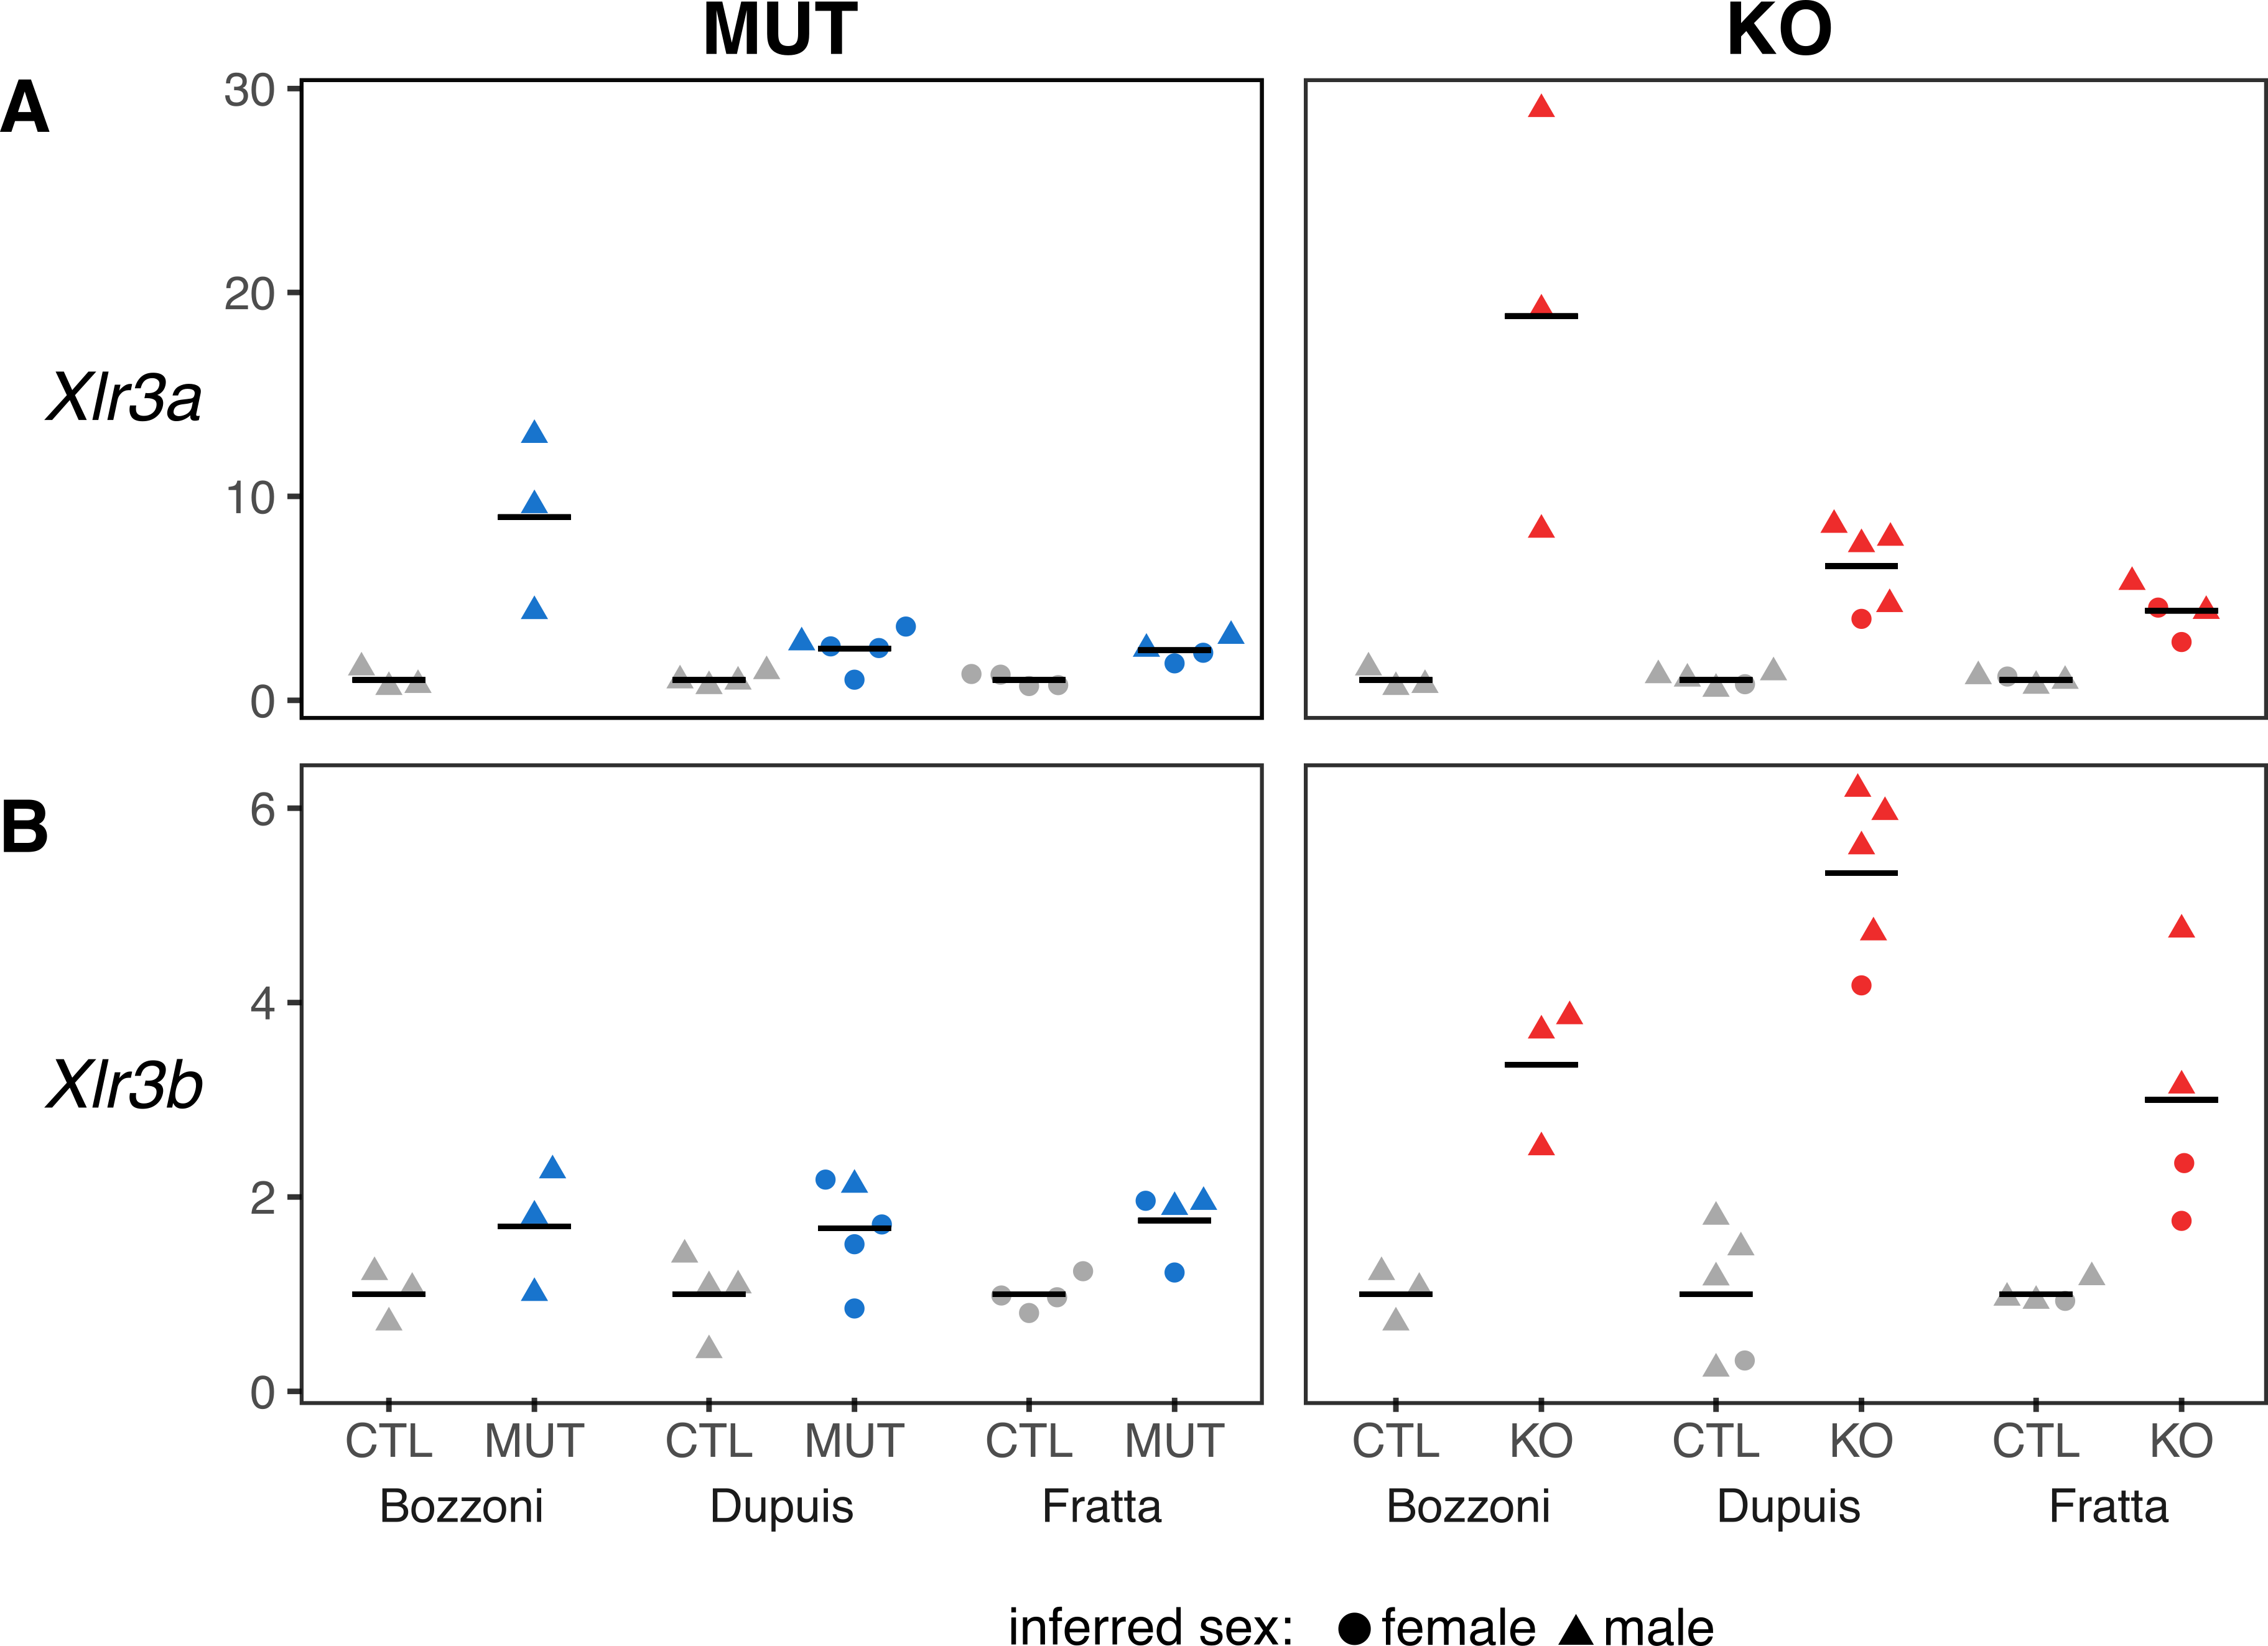
\includegraphics[width=10cm]{Figures/06_fus_meta/xlr_sex_expression.png}
	\caption{\textbf{Xlr genes are upregulated in both FUS KO and FUS MUT in mice of both sexes} }	
    Normalised read counts in each dataset, plotted relative to the mean of each dataset and condition-specific control group for Xlr3a (A) and Xlr3b (B). 
	\label{fig:fus_xlr_expression}
\end{figure}


%Comparing the log2 fold changes (LFC) between KO and MUT with linear regression demonstrates that the overlapping genes are changed on average 76\% in MUT of the strength in KO. ( lfc_MUT = 0.76 . lfc_KO - 0.0017; P < 1e-16; F-test).

% opposing 7 genes
%Only 7 genes are changed in the opposite direction (0.5%). 3/7 have FUS iCLIP peaks overlapping
%Prickle2 is a synaptic gene, large number of iCLIP peaks in first 250kb intron - long gene!
%Dcaf7 has a 7 read iCLIP peak in the first intron (short intron)
%Cds2 has 2 peaks (7 and 1) in the 3'UTR


\subsection{Synaptic and RNA-binding genes are a common gene expression response to FUS nuclear depletion}

\begin{figure}[h!]
	\centering
	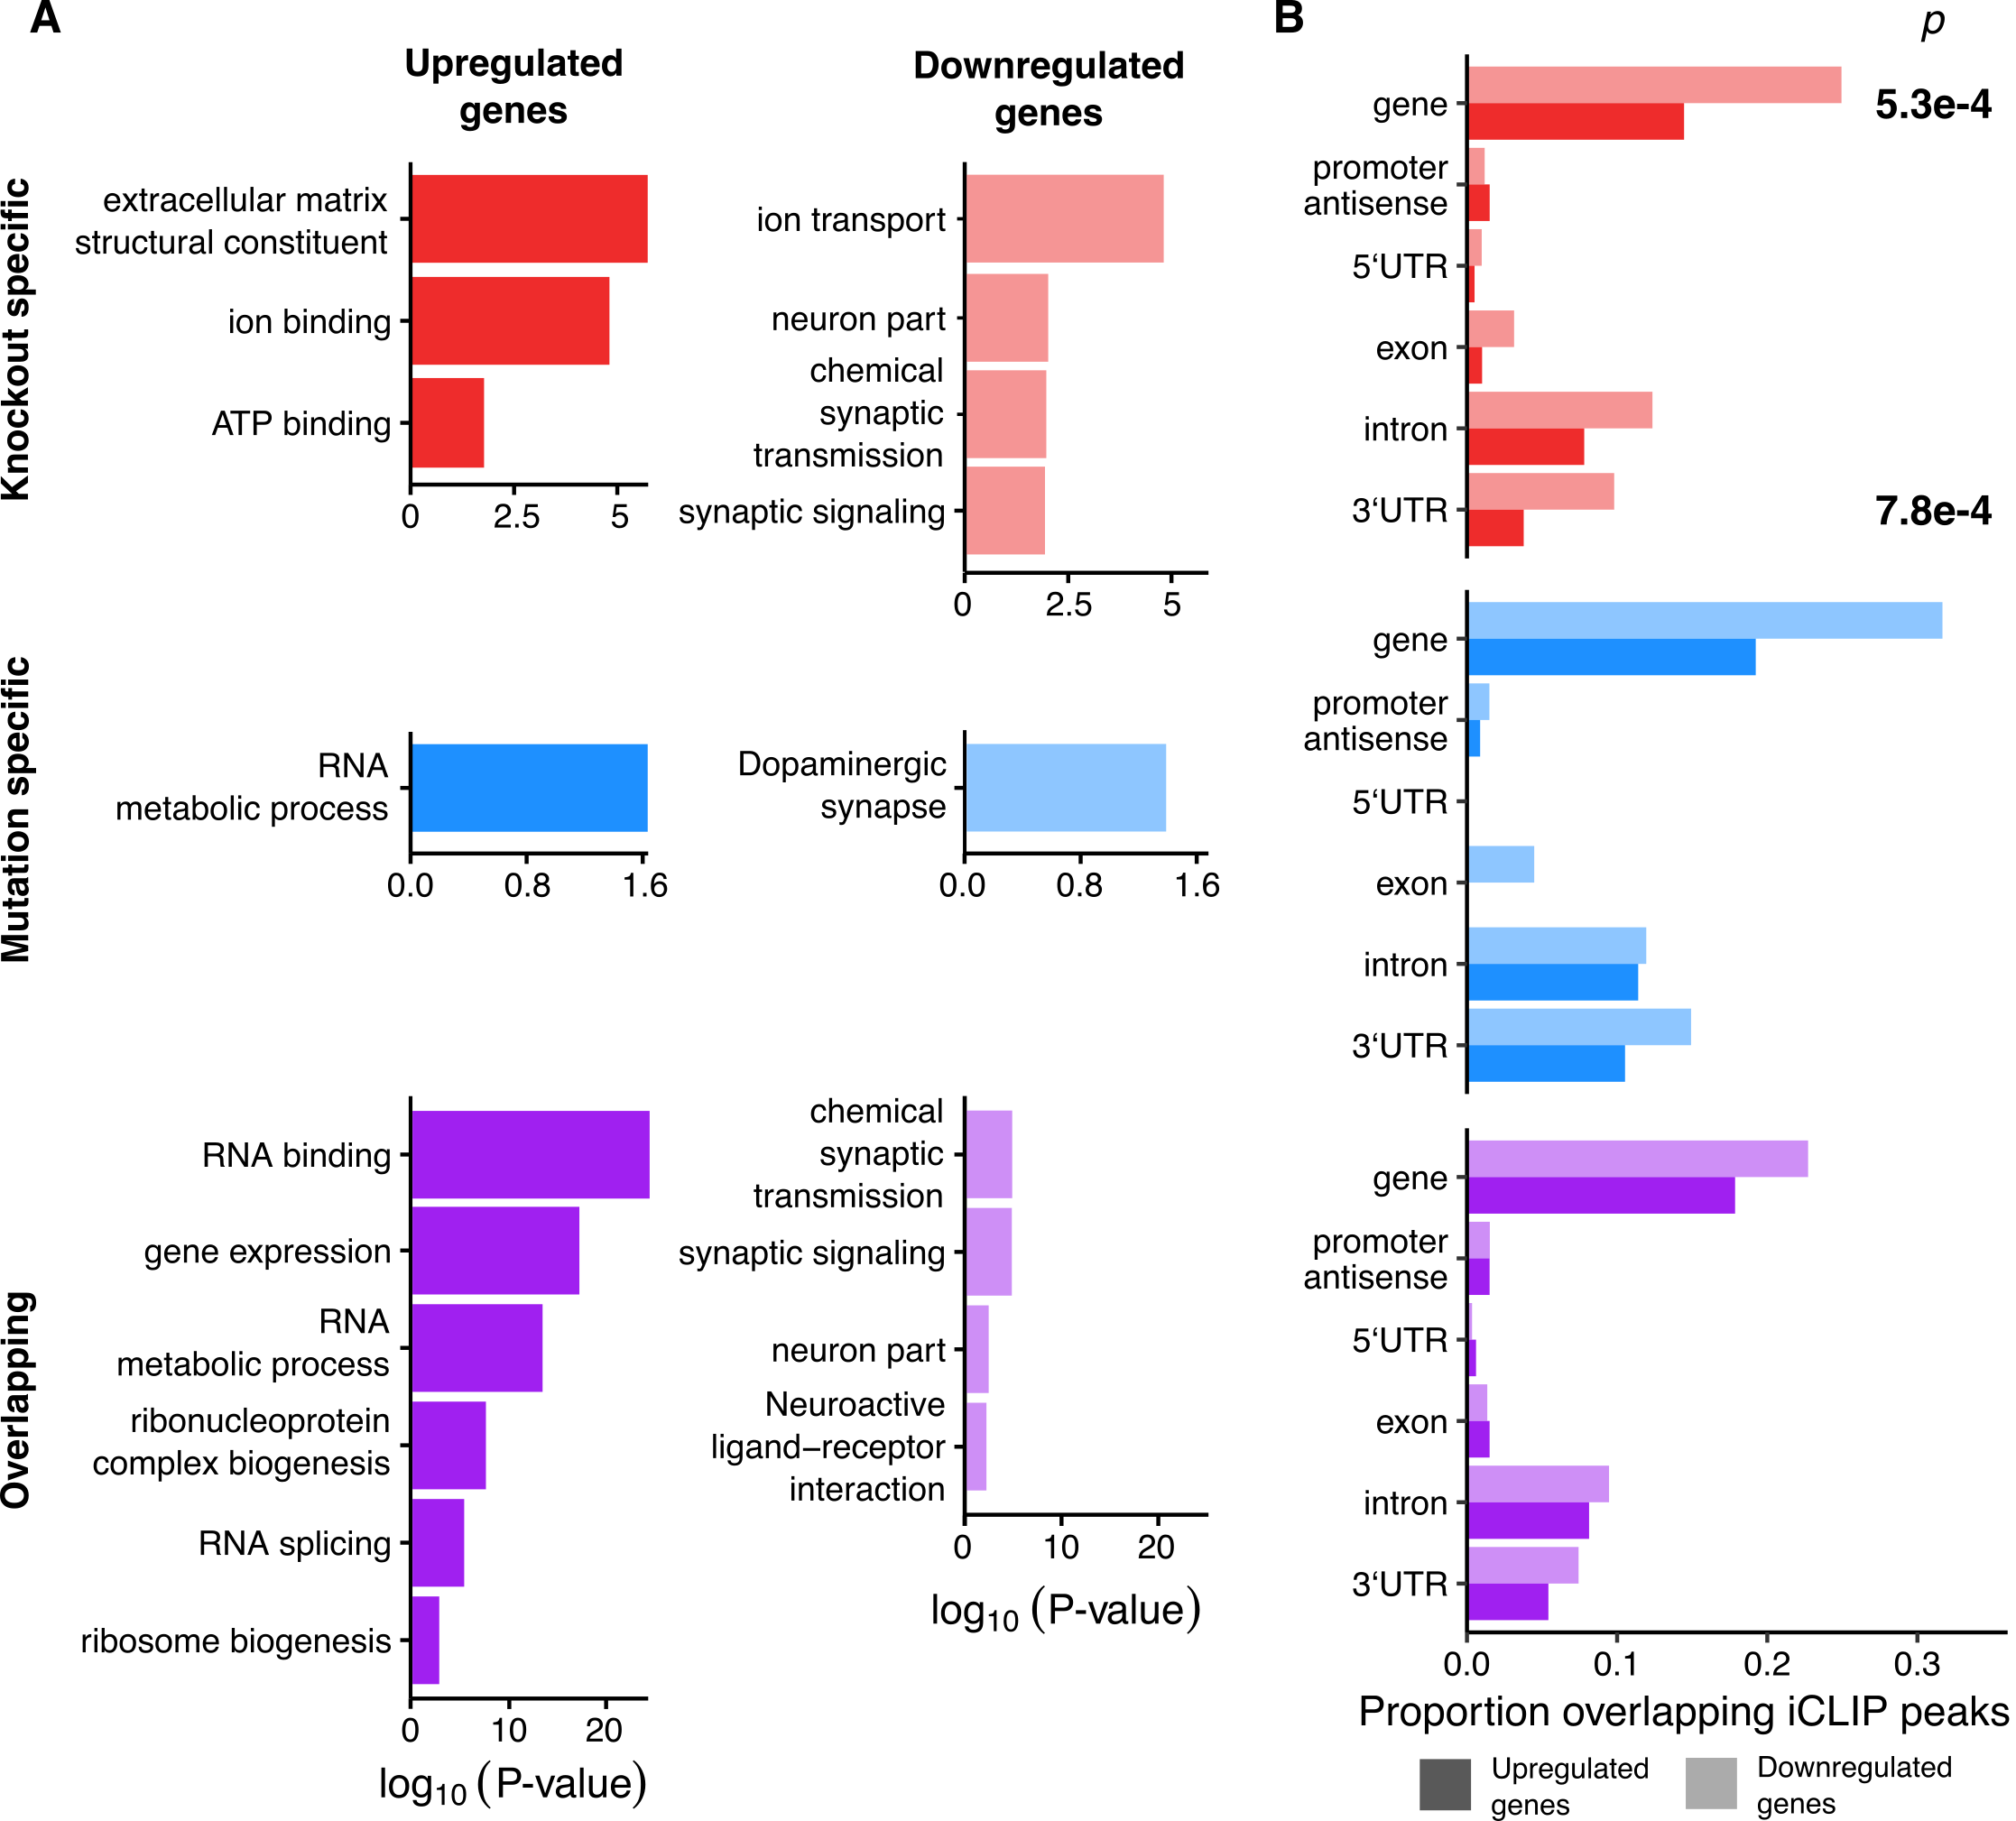
\includegraphics[width=\textwidth]{Figures/06_fus_meta/expression_curated_go_terms.png}
	\caption{\textbf{Overlapping genes are enriched in neuronal and RNA terms} }	
	A: Enriched Gene Ontology terms in the three groups of genes, split by direction.
	B: Proportions of each set of genes that have any iCLIP clusters within the entire gene or in any particular gene feature, split by direction. 
	P-values are from $\chi^2$ test of equal proportions. P-values presented are those below the Bonferroni corrected threshold of 0.05 / 18 = 0.0028. 
	\label{fig:fus_expression_go}
\end{figure}


Gene ontology (GO) terms enriched in the overlapping genes were strongly direction specific, with upregulated genes enriched in terms involving RNA binding, splicing and metabolism whereas downregulated genes were enriched in synaptic and neuronal terms (Fig. \ref{fig:fus_expression_go}A).
Knockout-specific and mutation-specific genes were less clearly enriched in specific functions. 
Knockout specific genes were involved in extracellular membrane functions, ion channels and amino acid transport whereas the mutant specific genes showed an enrichment in dopaminergic synapses and RNA metabolism.


\subsection{ Overlapping genes are bound by FUS in introns and 3'UTRs}

Individual nucleotide resolution crosslinking and immunopreciation (iCLIP) is an experimental technique for identifying the RNA targets of RNA-binding proteins. 
Using iCLIP and other RNA-protein interaction techniques, FUS has been shown to preferentially bind within introns and 3' untranslated regions (3'UTRs) rather than exons. \citep{Lagier-Tourenne2012-wa, Rogelj2012, Ishigaki2012, Masuda2015, Kapeli2016}. 
FUS binding at the 3'UTR has been shown to influence polyadenylation of certain genes \citep{Masuda2015} but may also have a role in directing mRNA localisation or competing with microRNAs, which in animals predominantly bind 3'UTR sequences to trigger degradation \citep{Lee1993,Carthew2009}.
A small number of genes have been reported to have FUS binding  sites upstream and antisense of the promoter, which correlated with upregulation of the gene upon FUS knockdown \citep{Ishigaki2012}.
I used the coordinates of FUS binding sites enriched relative to a background control in a published FUS iCLIP dataset from embryonic day 18 mouse brain \citep{Rogelj2012} to investigate a relationship between specific FUS binding and the direction of gene expression in the different gene sets.

The iCLIP binding profiles of the three sets of genes are similar with introns and 3`UTR sequences most commonly bound (Fig. \ref{fig:fus_expression_go}B).  
Comparing the proportion of upregulated and downregulated genes that change only in FUS knockout, there is an enrichment in iCLIP clusters in downregulated genes (P = 5.3e-4, $\chi^2$ test of equal proportions), an enrichment driven primarily by 3'UTR binding (P = 7.8e-4). 
This direction preference is not seen in the mutation-specific or overlapping gene sets.
Promoter-antisense binding is found in a small number of genes and at a similar proportion between gene set and direction of change.
As the iCLIP used is from predominantly nuclear wildtype FUS, any potential cytoplasmic interactions between NLS mutant FUS and spliced mRNAs cannot be observed.

% wrap up gene expression?

%% SPLICING

\subsection{FUS modulates the inclusion of a set of highly conserved RNA-binding protein introns}

I then used the same joint modelling approach to assess evidence of differing effects between FUS knockout and NLS mutation on alternative splicing.
For the individual analyses I used SGSeq \citep{Goldstein2016} to discover and quantify all possible alternative splicing isoforms, both novel and annotated. 
The read counts supporting each splicing variant were used to test for differential usage between conditions for either NLS mutation or knockout and their respective controls.
For the joint analyses, I ran SGSeq on all the samples simultaneously and then fit two separate models for all knockout samples and their controls (KO) and all mutation samples and their controls (MUT), incorporating a dataset-specific covariate. 
Models were fit using DEXSeq \citep{Anders2012}.
Table \ref{tab:splicing_results} summarises the numbers of splicing events in the KO and MUT models at FDR < 0.05.
%Here the weakness of the Dupuis samples for capturing splicing is revealed, presumably due to the short single-end sequencing reads. 
The joint models increased power as for MUT and KO respectively 93 and 890 events are found to be significantly altered, more than the sums of the individual analyses.
There is also a very good concordance between each individual analyses and their joint model, with the exception of the Bozzoni mutant samples (only 7 out of 31).

Comparing the joint FUS knockout and NLS mutation splicing models, the two overlap at both a strict and relaxed significance threshold.
With the relaxed overlap criteria only 16 splicing events remain specific to the NLS mutations (Fig. \ref{fig:fus_splicing_multi}A) .
There are 501 knockout specific splicing events and 405 that overlap between the two conditions.
Manual curation of the 16 mutant specific events gave little confidence of a mutation-specific effect on splicing, as only one splicing event appeared convincingly in all 3 datasets.
The single event that did appear to be real was an intron retention event in \textit{FUS}, far upstream of the mutated NLS region.

% TABLE OF SPLICING EVENT COUNTS
\begingroup
\renewcommand{\arraystretch}{1.5} 
\begin{table}[h]
	%\begin{centerline}
	\begin{tabular}{|r|ccc|ccc|}
		\hline
		%\centering
		& Bozzoni & Dupuis & Fratta & Bozzoni & Dupuis & Fratta\\[-0.3cm]
		& MUT & MUT & MUT & KO & KO & KO\\
		\hline
		Individual hits                & 47 & 1 & 79 & 275 & 54 & 316 \\
		Overlapping joint model & 9 & 0 & 33 & 143 & 31 & 206 \\
		Unique to dataset          & 38 & 1 & 46 & 132 & 23 & 110 \\
		\hline
		\textbf{Joint model}       & \multicolumn{3}{c|}{93} & \multicolumn{3}{c|}{890} \\
		\hline
		Overlap (strict)              & \multicolumn{2}{c|}{33} & \multicolumn{2}{c|}{\textbf{60}} & \multicolumn{2}{c|}{830} \\
		Overlap (relaxed)           & \multicolumn{2}{c|}{16} & \multicolumn{2}{c|}{\textbf{405} } & \multicolumn{2}{c|}{501} \\
		\hline
	\end{tabular}
	%\end{centerline}
	\caption{\textbf{Results from separate and joint splicing analysis}}
	\label{tab:splicing_results}
\end{table}
\endgroup

% types of splicing event - how many are annotated?
Comparing the different types of splicing event shows a similar distribution between knockout-specific and overlapping splicing events, both of which are dominated by complex splicing events.
These events are combinations of multiple types, such as a cassette exon accompanied by a retained intron and multiple alternative 3' and 5' splice sites, all within the same locus. 
When using tools like SGSeq that can pick up novel splicing events it can be expected that the majority of events are indeed complex. This has been seen with other splicing tools \citep{Vaquero-Garcia2016}.
An example of a complex event is in \textit{Ybx1}, which comprises a cassette exon within a retained intron  (Fig. \ref{fig:fus_splicing_multi}D).
The second largest category of event are retained introns.
An example of this class is seen in \textit{Ewsr1}, where a normally retained intron is less retained in both FUS knockout and NLS mutation (Fig. \ref{fig:fus_splicing_multi}E).
The third largest category are the cassette exons, which can either be skipped or included. 
An example is an annotated cassette exon in the neuronal gene \textit{Nrxn3}, which is included more in FUS knockout and NLS mutation when compared to wildtype (Fig. \ref{fig:fus_splicing_multi}F).
RNA-seq traces of all events mentioned above are in the appendices.
% expand on this or not?
Alternate 5' and 3' splice sites can be found in all three sets of genes, with alternate 5' sites appearing at twice the rate of alternate 3' splice sites. 
This discrepancy could be explained by the interaction of FUS with the U1 snRNP \citep{Yu2015a,Yu2015b}.
Knockdown or NLS mutation of FUS could lead to impaired U1 snRNP binding and hence disrupted 5' splice site recognition.


\begin{figure}[t]
	\centering
	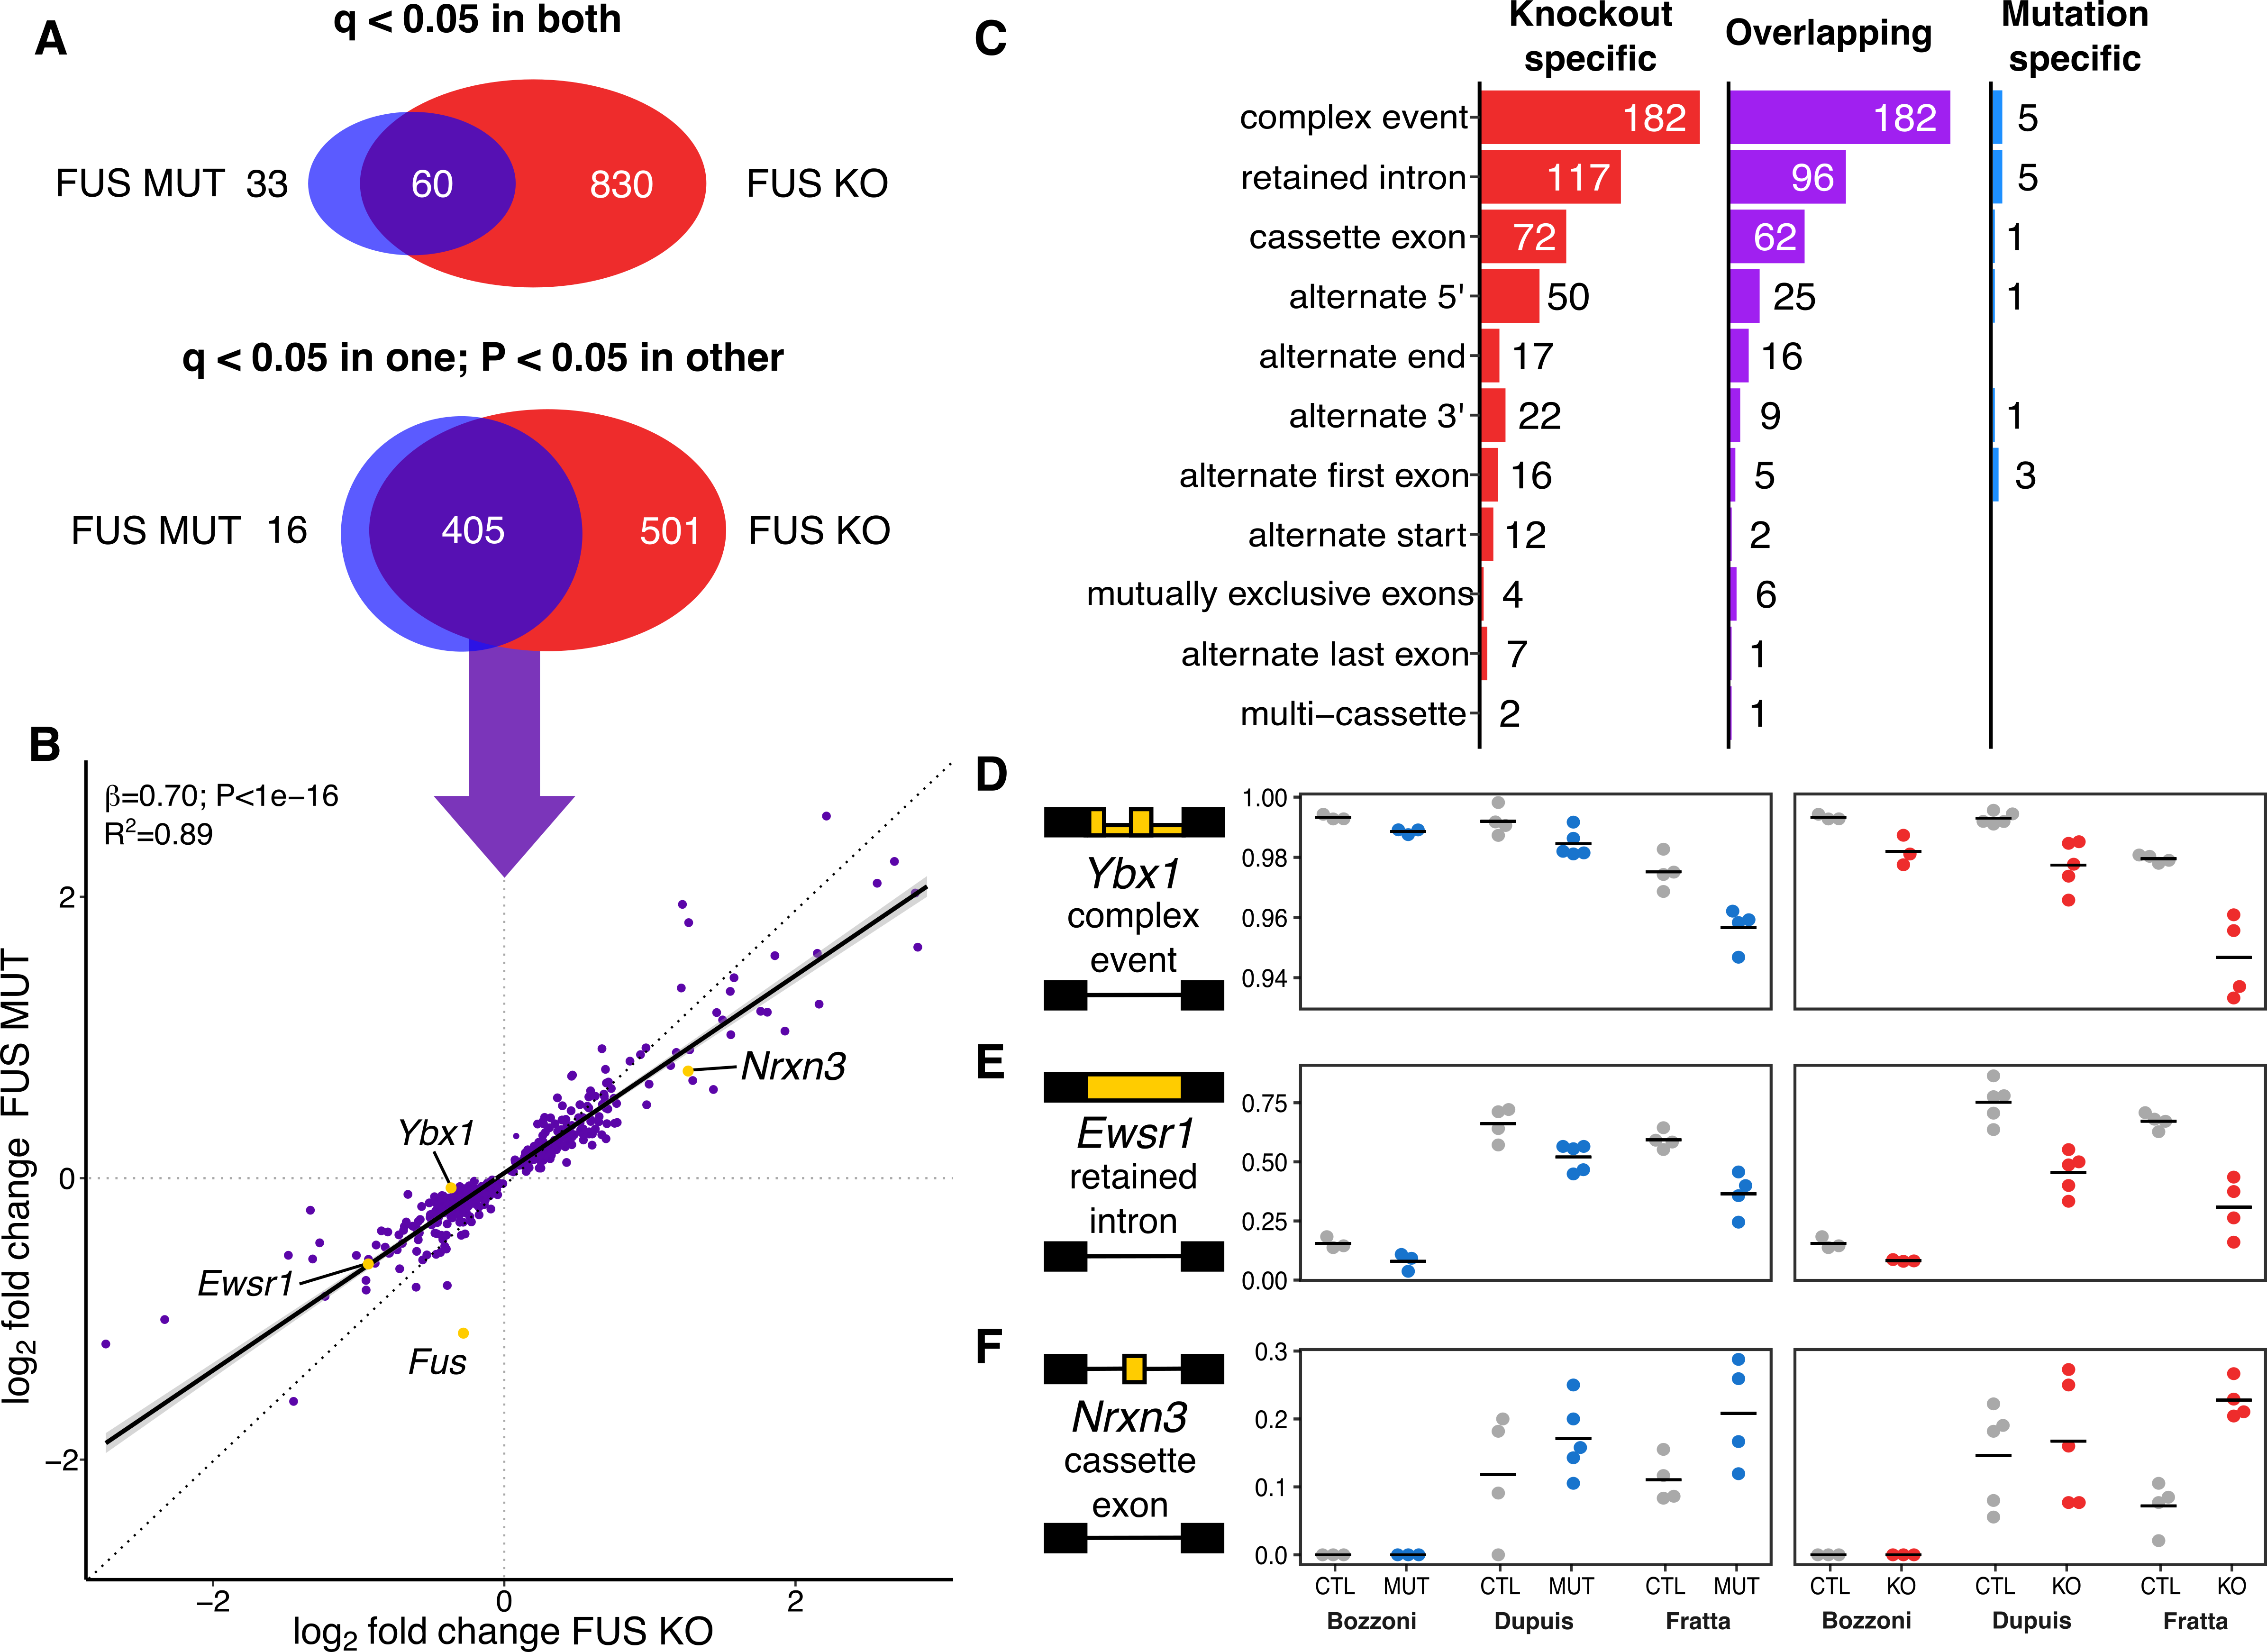
\includegraphics[width=\textwidth]{Figures/06_fus_meta/splicing_multi.png}
	\caption{\textbf{Splicing changes  strongly overlap between KO and MUT joint models}}
	A: Overlapping KO and MUT splicing events results in a significant overlap. The number of mutation specific events drops to just 16 when a more relaxed overlap threshold is used.
	B: Splicing events plotted by their $log_2$ fold change values in the KO and MUT joint models. There is a bias towards larger changes in the KO than MUT ($\beta = 0.7$; .P < 1e-16). Dotted line $y=x$; bold line fitted regression
	C: Categories of splicing variant found in each set of events. Complex events are defined as splicing events which are made up of multiple categories.
	D-F: Examples of a cassette exon, retained intron and a complex event in all three datasets. 
	\label{fig:fus_splicing_multi}
\end{figure}

Comparing the strict to the relaxed overlap criteria between the KO and MUT joint models reduces the number of events found to be specific to FUS mutation to 16, with 405 overlapping events and 501 found to be specific to FUS knockout (Table \ref{fig:fus_splicing_multi}). 
Plotting the $log_2$ fold changes of the overlapping splicing events, there is a similar trend towards larger fold changes in the KO than the MUT joint models ($\beta$ = 0.7, P < 1e-16; F-test; $R^2$ = 0.89). 
There are no overlapping splicing events that change in opposing directions between the two joint models.

\begin{figure}[t]
	\centering
	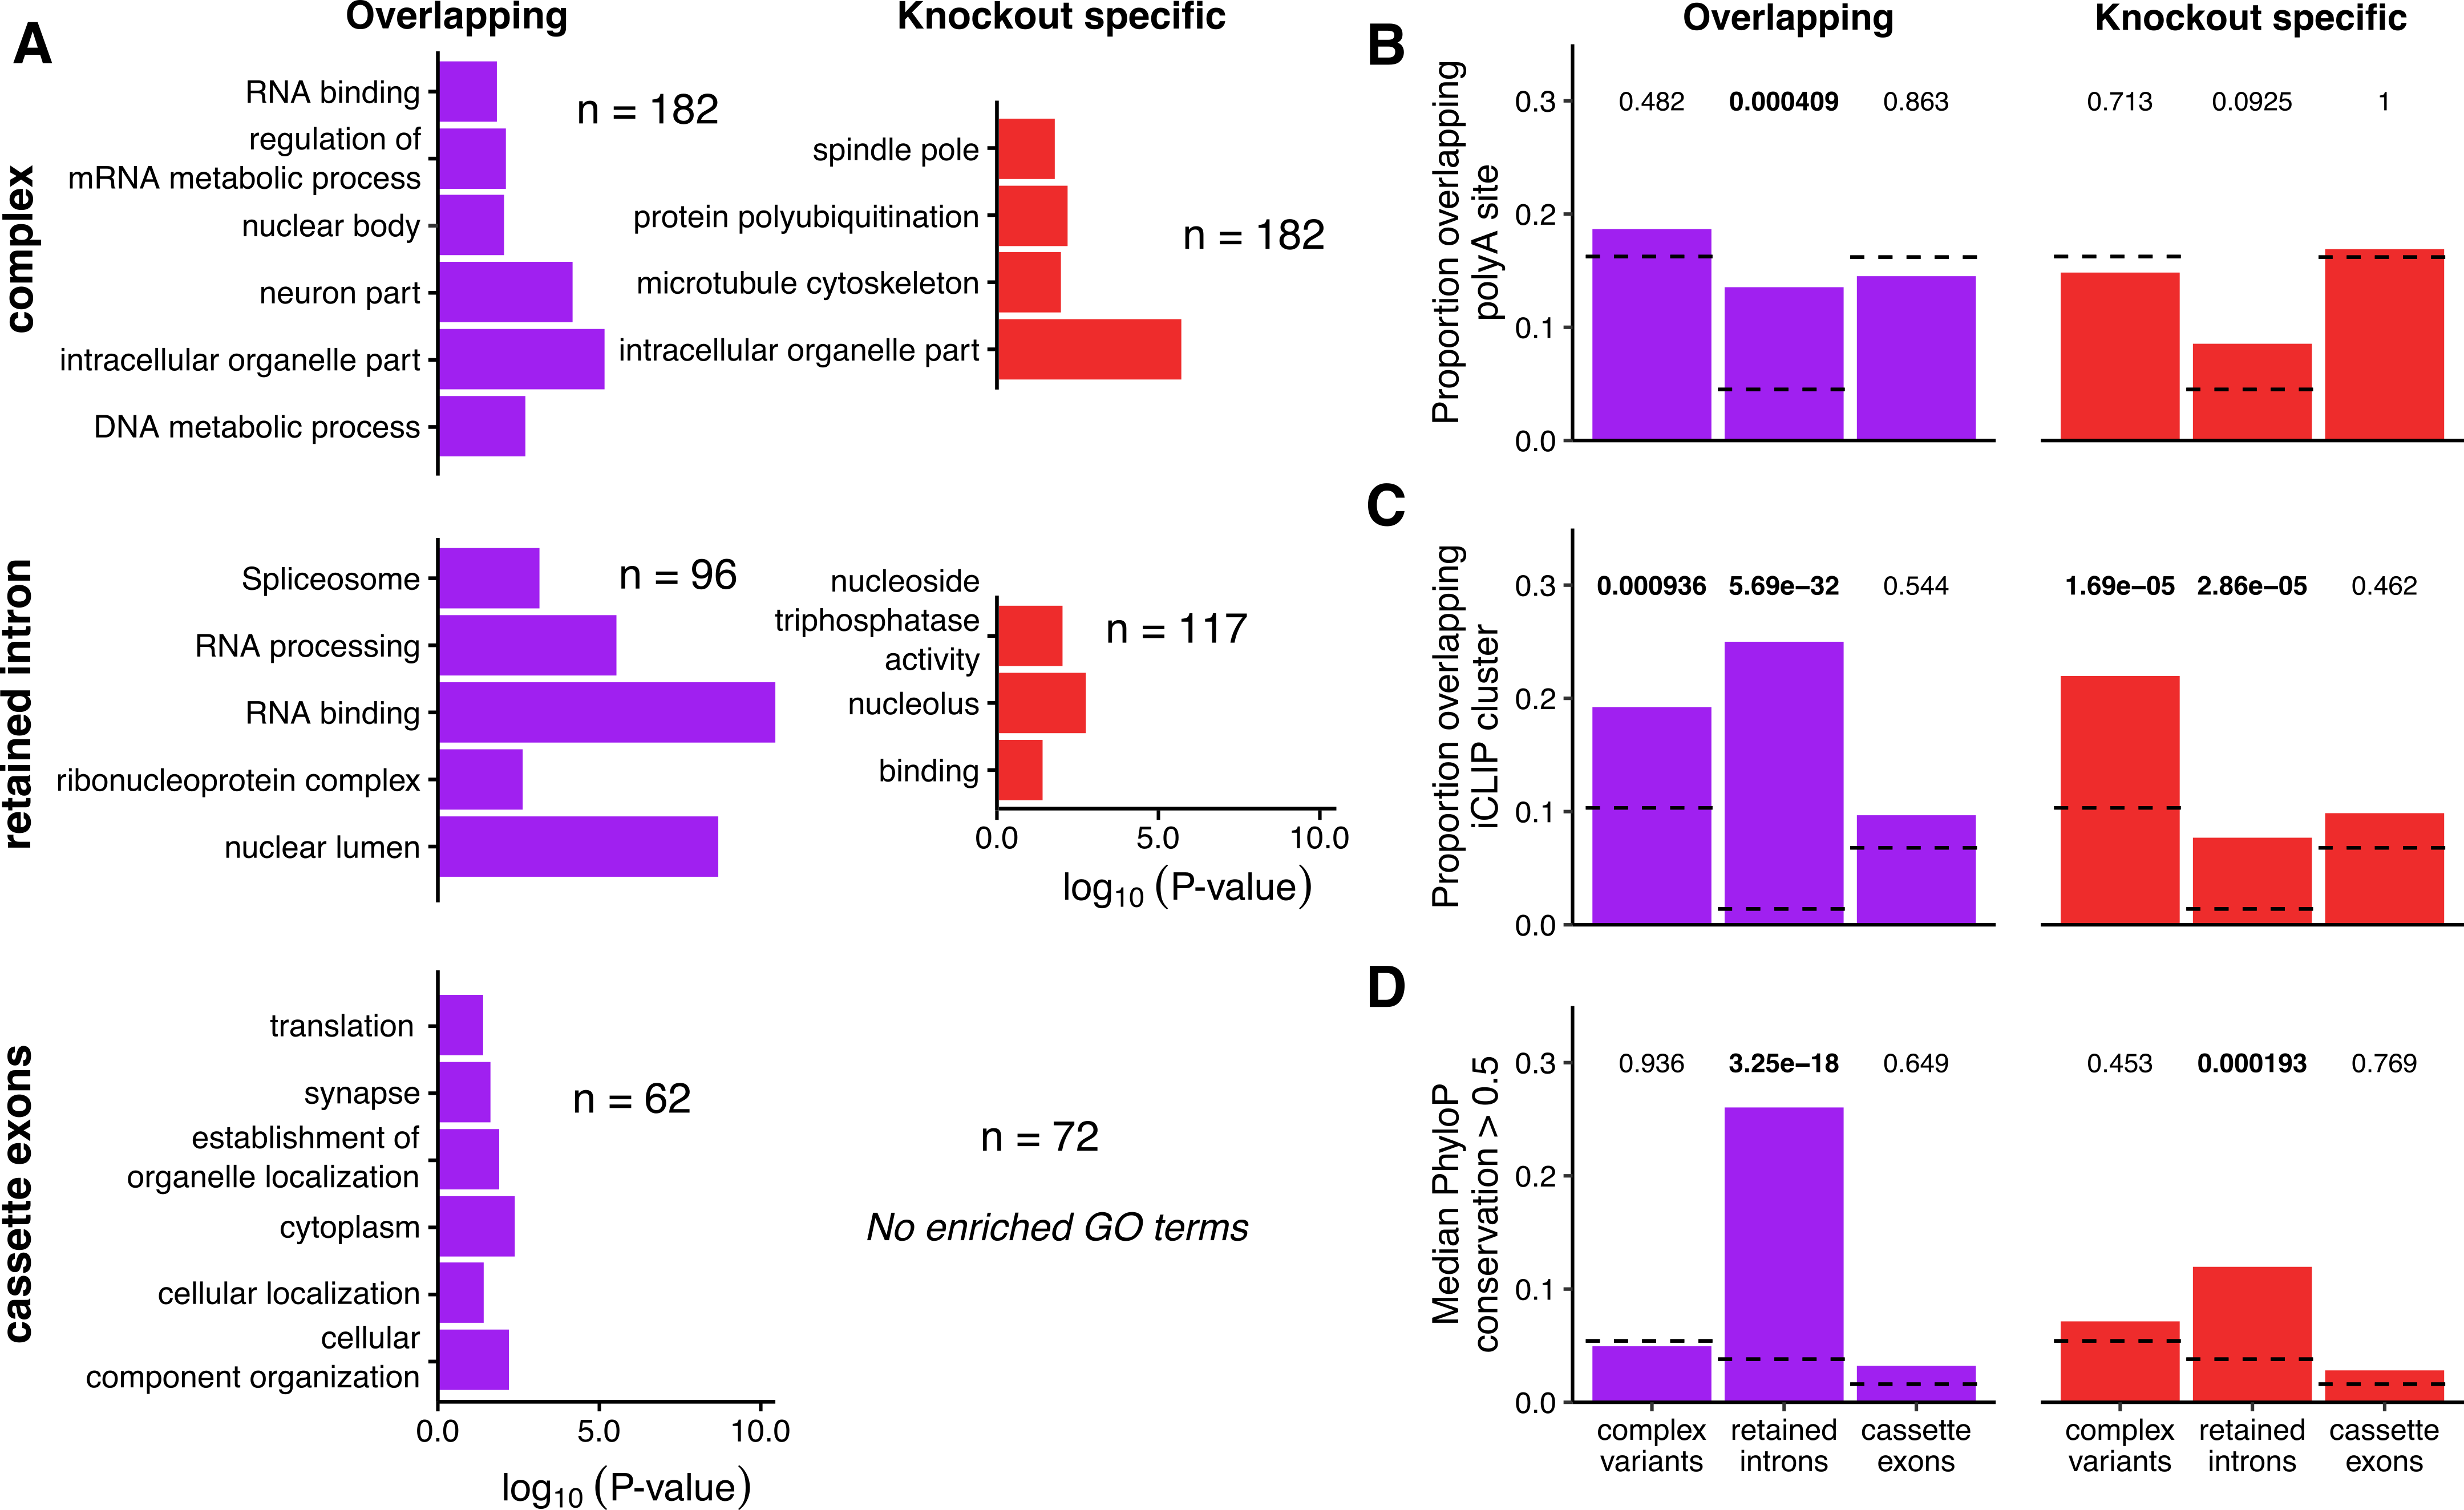
\includegraphics[width=\textwidth]{Figures/06_fus_meta/splicing_go_functions.png}
	\caption{\textbf{Intron retention events are highly conserved and occur in RNA binding proteins} }	
	A: Significantly enriched Gene Ontology terms found in genes split by category and splicing variant type.
	B: The proportion of each type of splicing variant in each category that overlaps a polyadenylation cleavage site.
	C: The proportion of each type of splicing variant in each cateoory that overlaps a FUS iCLIP peak.
	D: The proportion of each type of splicing variant in each category that have a median PhyloP conservation score greater than 0.5.
	\label{fig:fus_splicing_functions}
\end{figure}

The three largest categories of splicing events for the knockout-specific and overlapping events were complex, retained intron and cassette exons. 
I subjected each category to enrichment tests both for gene ontology terms and other genomic features.
There was a clear enrichment in RNA-binding and neuronal GO terms in the overlapping splicing events, with terms relating to RNA binding dominating retained introns (Fig \ref{fig:fus_splicing_functions}A). 
Conversely neuronal terms were found in cassette exons. 
Knockout-specific splicing events were enriched for different sets of genes, including microtubule and nucleolus.

The complex and intron retention events may arise from differences in polyadenylation site usage.
FUS has been observed to modulate polyadenylation \citep{Masuda2015}.
To investigate this I compared each set of splicing events with a set of annotated polyadenylation sites \citep{Gruber2016}.
Only overlapping retained introns were enriched for polyadenylation sites (P = 0.004), suggesting some intron retention events are mislabelled 3'UTRs (Fig \ref{fig:fus_splicing_functions}B).

Direct regulation of splicing events by FUS binding to introns has been proposed using RNA-protein interaction experiments \citep{Lagier-Tourenne2012,Rogelj2012, Ishigaki2012}.
To look for evidence of FUS regulating these splicing and polyadenylation events I used the same set of FUS iCLIP clusters from \citep{Rogelj2012}.
Complex events and retained introns were enriched in having iCLIP clusters within the affected introns in both overlapping and knockout-specific contexts.
The strongest enrichment was seen in overlapping retained introns (P = 5e-32; Fig \ref{fig:fus_splicing_functions}A). 
No enrichment was seen in cassette exons, suggesting that cassette exon splicing changes are not the direct result of a change in FUS binding.

RNA-binding proteins often contain intronic sequences that are very highly conserved \citep{Lareau2007} and these sequences are often used in the regulation of their translation \citep{Ni2007}.
To test whether the splicing events show high sequence conservation, I calculated the median PhyloP score using the 60-way comparison between mouse and other species for each encompassing intron \citep{Pollard2010-fj}.
Sets of events were then tested on the proportion of the set with a median phyloP score > 0.5, where a score of 0 is neutral and 1 is highly conserved.
Only retained introns were shown to be enriched in sequence conservation, and  at a greater externt for overlapping (P = 3e-18) than in knockout-specific events (P = 0.0002; Fig \ref{fig:fus_splicing_functions}D). 
For cassette exons the two flanking introns are included and so the median conservation score will reflect the conservation of those introns, even when the central cassette exon itself is highly conserved.

Taken together, these results show that nuclear loss of FUS through either knockout or NLS mutation leads to a set of splicing changes concentrated in conserved intron retention events affecting other RNA-binding proteins.
 Cassette exons do not tend to be bound by FUS beyond the null expectation and originate from less conserved introns.

% overlap splicing and gene expression
As the splicing events are enriched for similar gene ontology terms as the differentially expressed genes, I reasoned that these may affect the same group of genes.
However, only 59 differentially expressed genes are found to contain a splicing event. 
Of those 59, only 12 have FUS iCLIP binding peaks (17\%).
Those 12 genes all have either complex or retained intron events and includes the U1 splicing factor \textit{Snrnp70}, the FET protein family members \textit{Ewsr1} and \textit{Taf15}, and \textit{Fus} itself. 
This analysis shows that the role of FUS on gene expression and splicing mostly affects mutually exclusive sets of genes.


\subsection{FUS autoregulation is dependent on intron retention}

\begin{figure}[h!]
	\centering
	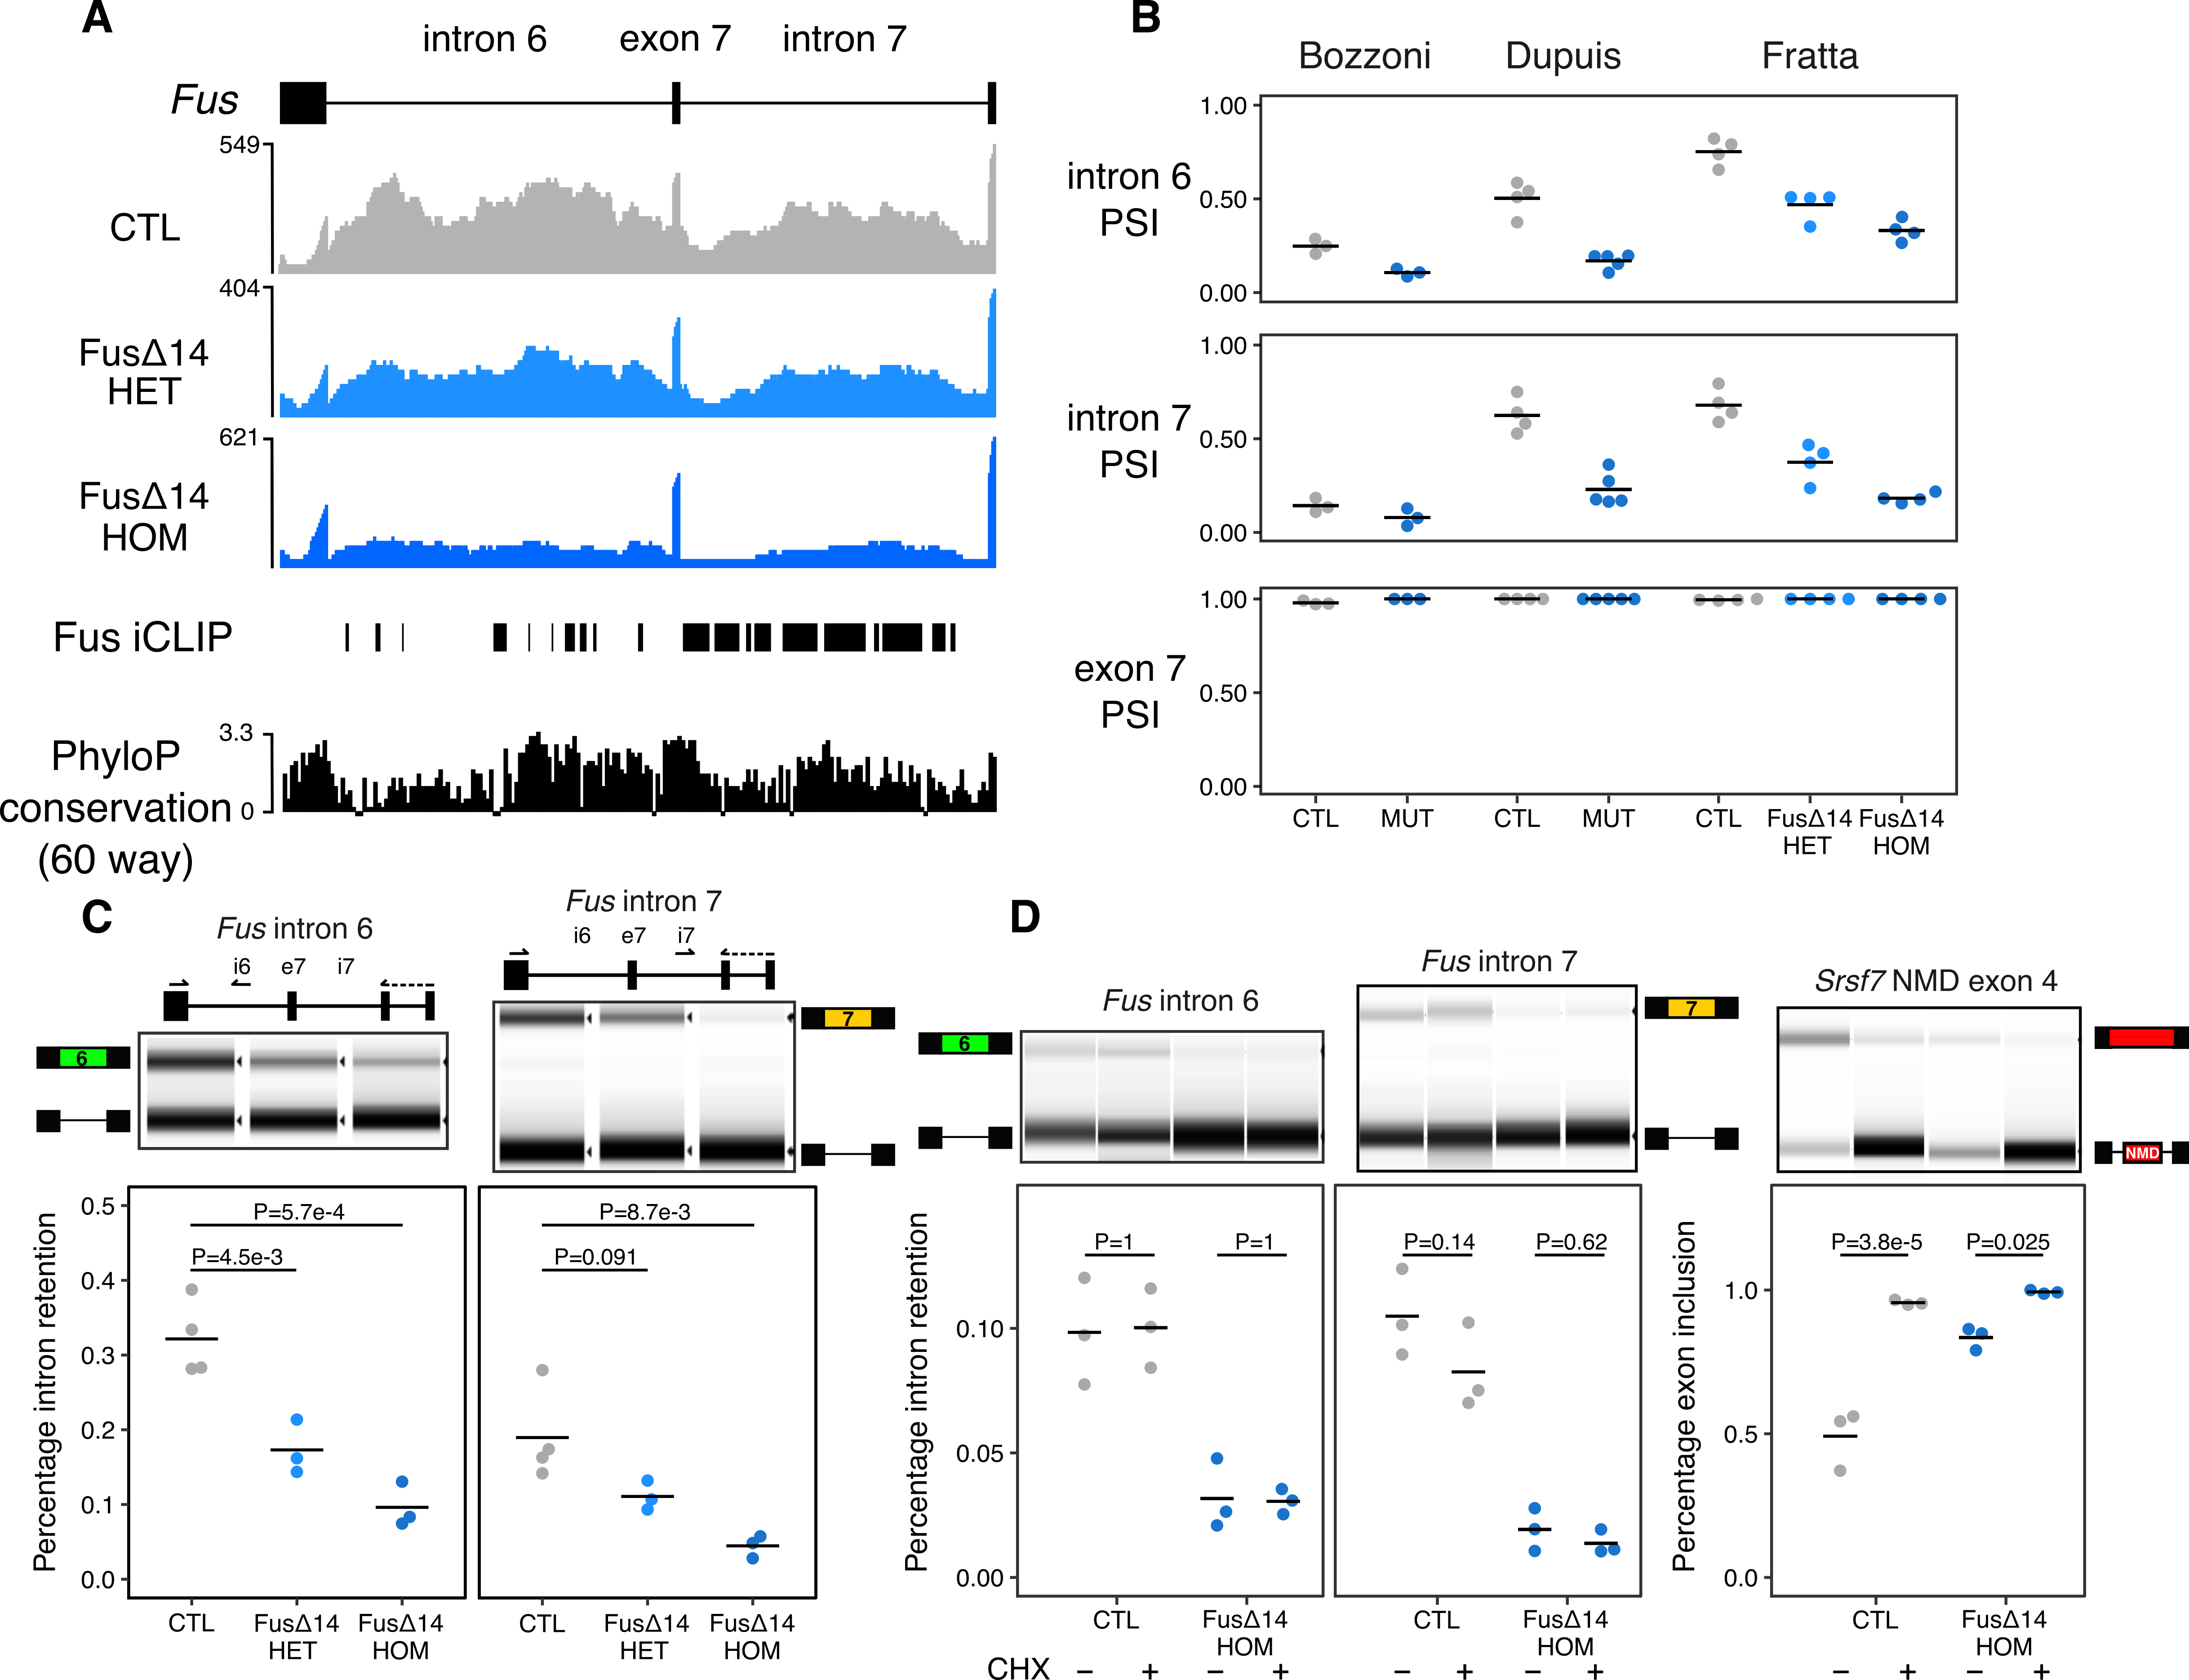
\includegraphics[width=\textwidth]{Figures/06_fus_meta/Fus_autoregulation.png}
	\caption{\textbf{Fus intron retention is an NMD-insensitive autoregulation mechanism } }
		A: FUS introns 6 and 7 are highly conserved and have multiple FUS iCLIP binding peaks. 
		Retention of introns 6 and 7 is decreased with increasing dose of the FUS $\Delta$14 mutation. 
		RNA-seq coverages for example wildtype, FUS $\Delta$14 heterozygous and FUS $\Delta$14 homozygous samples are accompanied by FUS iCLIP and PhyloP conservation (60 way) tracks.
		B: Percentage spliced in (PSI) values of intron 6, intron 7 and exon 7 in the three datasets, including the FUS $\Delta$14 heterozygotes.
		C: RT-PCR validation of the reduction in intron 6 and 7 inclusion with increasing dose of FUS $\Delta$14 mutation. 
		Left panel - FUS intron 6 (ANOVA genotype P = 5.1e-4; t-test CTL vs HET P = 4.5e-3; CTL vs HOM P = 5.7e-4)
		Right panel - FUS intron 7 (ANOVA genotype P = 8.5e-3; t-test CTL vs HET P = 0.091, CTL vs HOM P = 8.7e-3 )
		D:	Translation blocked with cycloheximide (CHX) to observe whether the intron retention transcript is sensitive to nonsense-mediated decay. 
		Left panel: FUS intron 6 retention is not altered with CHX treatment. ANOVA treatment P=0.96; genotype P=1.9e-5; t-test CTL untreated vs CTL treated P=1; HOM untreated vs HOM treated P=1.
		Middle panel: FUS intron 7 retention is unchanged by CHX treatment. ANOVA treatment P=0.10; genotype P=3.7e-6; t-test CTL untreated vs CTL treated P=0.14; HOM untreated vs HOM treated P=0.62.
		Right panel - \textit{Srsf7} exon 4, a known NMD target, is increased by CHX treatment. ANOVA treatment P=5.3e-4; genotype P=0.011; t-test CTL untreated vs CTL treated P=3.8e-5; HOM untreated vs HOM treated P=0.025.
		All reported P-values are corrected for multiple testing.
	\label{fig:fus_autoregulation}
\end{figure}


% explain FUS autoregulation
The joint splicing analyses found 5 intron retention events in FUS itself.
3 of these are knockout-specific and probably result from increased intronic reads in the partial Bozzoni knockout samples. 
However, The 2 remaining introns (introns 6 and 7) were also found in the FUS NLS mutants.
These introns overlap with a large number of FUS iCLIP binding peaks and could be the site of regulation of the \textit{Fus} transcript by the FUS protein.
Many RNA-binding proteins have the ability to bind their own RNA to control the level of their own translation, a phenomenon known as autoregulation \citep{Rosenfeld2002,Jangi2014a}.
When protein levels are high, protein-RNA binding shifts splicing towards the production of an non-coding isoform.
This is commonly through exposing transcripts to nonsense-mediated decay (NMD) \citep{McGlincy2008-wh}, by including an exon containing a premature stop codon as in HNRNP L and NOVA \citep{Rossbach2009,Dredge2005}, skipping a frame-preserving exon as in PTBP1 \citep{Wollerton2004}, or splicing within the 3'UTR as in TDP-43 \citep{Ayala2011}. 

RNA-protein interaction experiments have revealed a large cluster of FUS binding across introns 6 and 7 of the FUS gene \citep{Lagier-Tourenne2012}, both of which show very high sequence conservation between species.
This region was previously suggested to be the locus of autoregulation due to both an annotated cassette exon event in exon 7 and an a early polyadenylation transcript being present in transcript annotation databases (Ensembl, Refseq).
Skipping of exon 7 is predicted to cause a frameshift which should trigger NMD. 
Zhou and colleagues first investigated the mechanism of FUS autoregulation by inhibiting NMD and looking at changes in splicing of exon 7 \citep{Zhou2013}.
The exon-skipping transcript increased when FUS was overexpressed and decreased when FUS was knocked down, suggesting this splicing event to be the autoregulatory mechanism.
However this mechanism does not explain the high sequence conservation of the diffuse FUS binding pattern across introns 6 and 7 (Fig. \ref{fig:fus_autoregulation}A).
When examining RNA-sequencing coverage of the FUS gene in the Fratta, Bozzoni and Dupuis datasets, I could not observe any changes in the inclusion of exon 7 in any sample.
However I could observe a strong retention of both introns 6 and 7 that decreased in the presence of FUS NLS mutations. 
This phenomenon can be seen in all three datasets (Fig. \ref{fig:fus_autoregulation}B), despite the baseline level of retention in wildtype cells being highly variable. 
We generated RNA sequencing data from mice heterozygous for the $\Delta$14 NLS mutation. 
Comparing wildtypes, heterozygous and homozgous FUS $\Delta$14 samples showed that retention of introns 6 and 7 decreased with dose of the mutation (Fig. \ref{fig:fus_autoregulation}A/B) .

We designed an RT-PCR assay to validate the intron retention changes with a three primer method that could amplify a spliced transcript spanning \textit{Fus} exons 6-7-8-9 with a second band for either exon 6-intron 6 or intron 7-exon8. 
Intron retention decreased in a mutation dose-dependent manner (intron 6 P = 5.7e-4; intron 7 P = 8.7e-4; ANOVA; Fig. \ref{fig:fus_autoregulation}C).
We failed to detect a band corresponding to the skipping of exon 7 in any sample. 

Retaining two introns would be expected to cause NMD through premature stop codons, which are abundant in both intron 6 and 7. 
This has been proposed as the main degradation pathway for intron retention transcripts \citep{Wong2013}, although the  nuclear retention and elimination (NRE) has also been implicated \citep{Yap2013}. 
To test whether the intron retention FUS transcript undergoes NMD we reran the RT-PCR experiments after inhibiting translation in mouse fibroblasts with cycloheximide for 6 hours.
This should cause NMD to be inhibited as NMD requires transcripts to be bound to the ribosomes.
No effect on intron retention by cycloheximide treatment was seen in either wildtype or FUS $\Delta$14 homozygous fibroblasts (Fig. \ref{fig:fus_autoregulation}D).
As a positive control I used the inclusion of a known NMD-sensitive exon in \textit{Srsf7} \citep{Edwards2016}, which increased in both genotypes. 

These experiments suggest that depleting nuclear FUS protein downregulates the production of an intron retention transcript insensitive to nonsense-mediated decay. 




%Yap2013 - intron retention in neurons of terminal 3' introns detains neuronal-specific transcripts in the nucleus which are eventually degraded not by NMD but by RNA surveillance proteins. and then switch to splicing out and cytoplasmic transport when Ptbp1 levels change

% negative feedback mechanism
% protein homeostasis
% protein binds own mRNA
% changes in protein levels alters the splicing of the mRNA from a productive isoform to an isoform susceptible to nonsense-mediated decay, by skipping a frame-conserving exon, or by introducing a poison exon.
% iCLIP experiments have revealed that Fus binds a large section of its own mRNA spanning ~ 3500bp comprising intron 6, exon 7 and intron 7. 
% Both introns show very high conservation between species, suggesting an important regulatory role for the introns.
% \cite{Zhou2013} and colleagues used RT-PCR to show that changes in FUS protein levels alters the inclusion of exon 7 and the exon 7-skipped transcript is sensitive to nonsense-mediated decay.
% Inspecting the RNA-seq traces from our data as well as Dupuis and Bozzoni, we see no evidence for any change in exon 7 inclusion in the presence of NLS mutated FUS.
% Instead we see a clear reduction in the retention of introns 6 and 7.
% Using RNA-seq data from the heterozygous FUS $\Delta$14 mice it is clear that the reduction in intron retention is dependent on the mutation dosage.

% To validate the intron retention changes I developed an RT-PCR assay with primers targeting exon 6 and exons 8/9 to selectively amplify spliced FUS mRNA and an additional third primer targetting either intron 6 or intron 7. This three primer PCR amplifies bands corresponding to intron 6 and 7 retention and splicing. Our primers did not amplify a band corresponding to exon 7 skipping. 
% With increasing dosage of the FUS $\Delta$14 mutation the proportion of intron retention reduces for both intron 6 and intron 7 (Figure \ref{fig:fus_autoregulation}C).

\section{Discussion}

% Reiterate what I've done and seen
This study is the largest transcriptome-wide assessment of FUS function to date.
By combining three separate datasets of FUS knockdown and NLS mutation I have been able to discover a large repertoire of differentially expressed genes and differential splicing events that have not previously been reported.
Comparison of the two conditions demonstrates that NLS mutations predominantly act to reduce nuclear FUS, as the majority of expression and splicing changes overlap and change in the same direction.
This leaves only a small number of NLS mutation-specific gene expression changes and almost no mutation-specific splicing changes other than in FUS itself. 
By studying the mutation-specific splicing changes in FUS I have discovered a novel intron retention transcript that could explain the mechanism by which FUS regulates its own translation.

The joint modelling approach has allowed me to combine three different RNA sequencing datasets to produce a consensus set of RNA phenotypes.
Due to the stochastic nature of transcription and splicing combined with the small sample sizes employed, these datasets are inherently variable.
By combining repeated observations  under the same genetic conditions we can better discover true FUS-associated changes.
While joint modelling increases detection power, it rewards conformity between experiments and I cannot discount the possibility that each dataset has its own cell-type or mutation-specific effects confounded with the dataset itself.
It is arguable that these dataset-specific changes are more likely than not to be biologically irrelevant such as transgene insertion artefacts. 
In addition, with increased power I can now detect changes in expression and splicing at very small effect sizes. 
While this provides more information, the biological relevance of these small changes is harder to investigate.
These changes are less likely to be a direct result of FUS RNA or protein interaction and may emerge through multiple downstream effectors or pathways.
%As a disease-associated protein, FUS has been intensely studied and the number of putative roles it has within the cell is large.  

Employing a relaxed significance threshold demonstrated that the majority of changes are shared between  FUS knockout and NLS mutation.
The direction of change was identical for 99\% of overlapping genes with a clear bias towards stronger changes in the knockout (Fig. \ref{fig:fus_expression_multipanel}B). 
This is unsurprising, as NLS mutations do not completely abolish FUS nuclear import \citep{Scekic-zahirovic2016, Devoy2017}.
% neuronal gene loss
There is a widespread downregulation of neuronal and synaptic genes in FUS nuclear depletion. 
This could be due to defects in RNA transport as FUS has been found in RNA transport granules \citep{Kanai2004, Fujii2005}.
% splicing factor upregulation
Conversely, RNA binding genes were upregulated in both conditions. 
FUS is known to interact on a protein-protein level with multiple splicing factors \citep{Yang1998,Meissner2003, Groen2013} and particularly members of the U1 snRNP complex \citep{Sun2015a, Yu2015a}. 
CLIP experiments show that FUS binds a number of these factors at the RNA level \citep{Nakaya2013}.
Therefore FUS is part of a complex network of RNA and protein interactions with multiple splicing factors. 
However, why FUS loss acts to upregulate these factors is yet to be discovered.
% Xlr genes
I managed to replicate the finding of upregulation of the X-linked lymphocyte receptor (\textit{Xlr}) cluster of genes, first seen in adult FUS knockout mice \citep{Kino2015}, suggesting that FUS loss causes chronic dysregulation of these genes. 
As Xlr gene overexpression can alter dendritic spine growth and are regulated by the Cux1/2 transcription factors \citep{Cubelos2010}, the mechanism of how FUS loss leads to their upregulation is intriguing. 
No FUS iCLIP clusters were observed overlapping any Xlr gene, discounting direct post-transcriptional regulation.
As these genes appear to be mouse-specific they are not directly relevant to disease but could provide a useful model for the effect of FUS on transcription.

% Splicing
Overlapping the joint splicing models demonstrated that almost all splicing changes attributed to NLS mutations could also be observed in FUS knockouts.
I did not observe a convincing set of mutation-specific splicing changes which is unsurprising as splicing is a nuclear function. 
The overlap between knockdown and expression has been seen in cells where overexpression of NLS mutant FUS cannot rescue splicing changes in FUS knockdown cells \citep{Sun2015a}.
Due to the multiplicity of FUS interactions between multiple splicing factors, disturbance of any or all of these factors could be confounding the splicing changes. 
For example, the splicing profiles of FUS NLS mutations overlap those from knockdowns of known interactor SMN \citep{Mirra2017}.
I observed approximately double the number of 5' splice site changes than 3' splice site changes. 
This could be due to the shorter length of the consensus 5' splice site sequence compared to the 3' making cryptic splice sites more likely by chance, but it may hint at a consequence of the interaction between FUS and the U1 snRNP.
Although the interaction between FUS and the U1 snRNP has been well studied \citep{Nakaya2013,Yu2015a,Yu2015b}, my analysis has uncovered a large array of splicing events to study the role of FUS in splicing.

The dominance of retained introns and complex events (where multiple splice sites are altered simultaneously) points to a more nuanced picture of splicing changes than has previously been investigated in RNA-binding protein biology.
I concede however that the large number of complex events seen in the joint splicing models is probably a result of the juction-centric method I used, as well as analysing all the data jointly. 
An isoform-centric approach where reads are assigned to specific transcripts \citep{Trapnell2010,Bray2016} perhaps would more sensitively tease out the different changes that are happening in complex introns.

% SPLICING AND TRANSCRIPTION - REWRITE

Nevertheless, complex events as well as intron retention events are enriched in FUS iCLIP binding and are more likely to affect splicing factors than the cassette exons I observed. 
This suggests a more subtle role for FUS in splicing than simply altering alternate cassette exons which have been the focus on previous studies on FUS and splicing \citep{Rogelj2012,Lagier-Tourenne2012,Ishigaki2012,Honda2014,Scekic-zahirovic2016}.
FUS can bind the C-terminus of RNA polymerase II \citep{Schwartz2012} and a study on the role of FUS in alternate polyadenylation suggested that FUS binding to pre-mRNA can stall RNA polymerase II \citep{Masuda2015}. 
Transcriptional speed is known to affect splicing as pausing transcription can allow more time for splicing factors to bind weaker affinity sequences \citep{Kornblihtt2004a}. 
Splicing events altered when transcriptional elongation is reduced are enriched for RNA binding genes \citep{Ip2011}. 
This suggests that the intron retention events seen in FUS knockout and mutation, including \textit{Fus} itself may arise from FUS stalling RNA polymerase II.

The high sequence conservation seen in retained introns suggests a regulatory role for these splicing events, despite the unexpectedly low overlap between splicing changes and differentially expressed genes.
One example of this is the U1 splicing factor \textit{Snrnp70}, whose highly conserved intron retention transcript has previously been shown to increase in FUS knockdown, which should lead to increased degradation of \textit{Snrnp70} mRNA through nonsense-mediated decay \citep{Nakaya2013}. 
Two overlapping splicing events are found in \textit{Snrnp70} that suggest the NMD-sensitive conserved intron section is more retained in FUS knockout. 
I observed upregulation of \textit{Snrnp70} in the FUS knockouts, although this gene-level metric may confound the change in isoforms suggested by the splicing analysis. 
The other FET family members \textit{Taf15} and \textit{Ewsr1} are both upregulated and both contain conserved intron retention events that are more frequently skipped in FUS depletion.
For \textit{Taf15}, its upregulation when FUS is depleted is probably a redundancy mechanism due to the shared RNA motifs and target genes of the two proteins \citep{Ibrahim2013,Kapeli2016}. 
The splicing changes I identify in both \textit{Taf15} and \textit{Ewsr1} suggest a mechanism for how their expression is increased when  nuclear FUS is depleted.
A previous study did not find the mRNA stability of \textit{Taf15} to be changed in FUS knockdown \citep{Colombrita2012} but this requires re-evaluation in light of the new data.

By studying our RNA-seq data in all three NLS mutant datasets I observed a novel intron retention isoform whose retention inversely correlates with the dose of NLS mutation. 
As the change can also be observed in mice heterozygous for the FUS knockout allele it is unlikely to be due to the mutant NLS itself (data not shown).
Although cassette exon skipping of exon 7 was previously suggested to be the splicing event of FUS autoregulation \citep{Zhou2013}, neither our RNA-seq or RT-PCR observed exon 7 skipping in the presence of NLS mutation.
This could simply be due to exon 7 skipping being present but at much lower level than intron retention changes. 
Zhou and colleagues could not have detected intron retention changes as the length of the retention transcript exceeds the maximum amplicon length for PCR. 
Our three-primer approach robustly demonstrated the changes in retention occur in both introns 6 and 7 but they cannot conclusively prove simultaneous retention of both introns. 
% Premature polyadenyaltion?
This would require a long-read sequencing technique. 
The NMD inhibition experiments suggest that the FUS intron retention transcript is insensitive to nonsense-mediated decay. 
Although, cycloheximide inhibits translation in order to inhibit NMD and off-target target effects cannot be excluded. 
To elucidate this as the mechanism of FUS regulation, further experiments are needed to validate this in human cells.
One possible mechanism is that the transcript is instead detained in the nucleus.
This is a regulatory pathway proposed for intron retention transcripts to prevent translation \citep{Boutz2015}.
A analogous mechanism for autoregulation has been proposed for TDP-43, where the binding of TDP-43 protein to \textit{Tardbp} mRNA shifts polyadenylation to create a long 3'UTR transcript which is detained in the nucleus and degraded by the exosome. The long transcript can also be spliced to form NMD-sensitive isoforms which can be exported to the cytoplasm and then degraded \citep{Ayala2011,Koyama2016}. It is unclear why the system would require two separate degradation pathways. 
In the light of this, the discovery of the FUS intron retention transcript could be a complementary mechanism to the one set out by Zhou and colleagues.
This would then answer the outstanding question of the high evolutionary conservation of both introns and the length of FUS binding throughout.

% ALS biology implications
This study combines multiple RNA sequencing experiments to better understand and catalogue changes in gene expression and RNA splicing in response to FUS nuclear depletion.
My analysis suggests that these changes are shared due to the extreme overlap and concordance of direction of gene expression and splicing.
It does not conclusively link any of these alterations to motor neuron toxicity and degeneration, which is only seen in NLS mutant embryos and not in FUS knockouts \citep{Scekic-zahirovic2016}.
It is unclear whether toxicity can be attributed to the 186 mutation-specific genes due to the sharing of gene ontology categories with the overlapping set (RNA processing and synaptic genes). 

The discovery of a novel mechanism for FUS autoregulation is valuable for understanding the role of FUS in disease.
Autoregulation acts to maintain protein homeostasis but FUS NLS mutations interfere with this.
When FUS nuclear import is abolished by mutations, there is no way for FUS protein to regulate  its own translation, leading to ever-more cytoplasmic FUS.
High concentrations of cytoplasmic FUS increase the likelihood for aggregation which NLS mutant FUS is more prone to do \citep{Bosco2010}. 
This is increased propensity maye be due to the recent finding that NLS acts to solubilise FUS aggregates through binding to Transportin \citep{Guo2018,Yoshizawa2018,Hofweber2018}.
In FUS ALS, patients only have a single copy of NLS mutant FUS. 
Selectively removing the mutant copy, at either a DNA or RNA level, should all but prevent cytoplasmic mislocalisation while maintaining nuclear FUS levels due to the compensatory nature of autoregulation. 
Indeed, mice heterozygous for a FUS knockout allele have FUS mRNA and protein levels at 75\% of wildtypes and exhibit no motor neuron degeneration \citep{Scekic-Zahirovic2017}. 
This could feasibly be increased to 100\% by modulating FUS autoregulation by promoting the splicing of introns 6 and 7. 
This work expands our understanding of the complex role of FUS in gene expression and splicing and uncovers a new model for FUS autoregulation. 
I hope this will be useful to the disease field in designing targeted therapies for FUS ALS.

% Largest transcriptome-wide study of FUS function to date
% Discovered a large number of differentially expressed genes and differential splicing events
% Discovered a novel mechanism for FUS autoregulation via intron retention.

%% Joint modelling

% Importance of replication
% RNA is inherently noisy
% Joint modelling provides clarity

% Joint models boost power but they reward conformity between datasets
% There may be important biological differences, such as subtle cell type or developmental differences that account for different genes and splicing events ocurring in different datasets

% Between sample variance clearly important to detecting RNA changes
% Unexplained why such a difference
% Any evidence of a polyA / total RNA effect on variance?

%% Gene expression
% We find the largest set of gene expression changes associated with FUS depletion.
% Knockout and NLS mutation have a strong overlap that is biased towards the knockout
% This makes biological sense as NLS mutations don't completely ablate nuclear import
% 99% of genes go in the same direction but 7 genes are upregulated in the FUS mutant
% P values are unconvincing but 3/7 have FUS binding so could be real, worth following up



% full-blown nuclear FUS depletion would only occur at disease endpoint
% adult loss of FUS is not toxic to motorneurons but would cause many changes in splicing factor biology
%  single copy FUS NLS mutations are still highly toxic


% We see more 5' changes than 3', implicating U1 impairment
% How many of the intron retention changes are due to U1-sensitivity? Are retained introns more sensitive to spliceosomal changes?

% No convincing splicing changes found to be mutation specific
% not surprising as this should be a nuclear function of FUS

% Retained introns are enriched for RNA binding function and FUS binding
% Previously seen for Snrnp70 - U1 factor
% This makes sense as FUS can interact with the whole U1 snRNP
% We have extended this to a larger group of proteins

% Cassette exons are not, this is surprising
% Boris found enrichment of FUS peaks within 200bp  of cassette exons whereas we took the entire intron and found no enrichment. Targeted appraoch is probably better.
% FUS's role in alternative exon splicing perhaps overstated

% Retained introns in RNA binding proteins suggests NMD mechanisms
% FUS is part of network of splicing factors that all cross-regulate
% Not surprising that mislocalisation of FUS triggers changes in other factors
% Taf15 and Ewrs1 obvious candidates to replace FUS, redundancy in system

% Complex events inherently difficult to interpret
% Here an isoform-level approach would be more effective
% Caveat is when one is interested in novel isoforms, as are important in TDP biology (cite my papers)

% theme - FUS alters splicing and gene expression of genes coding for proteins that FUS is known to interact with - U1 snRNP, hnRNPs, FET proteins, YBX1 \citep{Groen2013}.


%% Autoregulation 
% We have identified a new mechanism for FUS autoregulation
% Is it prematurely polyadenylated?
% RT-PCR primers are targeting isoform with exon 9 included which should be downstream of any premature polyadenylation site.

% why don't we see the Zhou exon 7?
%% No evidence from RNA-seq so skipping transcript may just be very lowly expressed.
% They wouldn't pick up intron retention due to being too long to amplify by RT-PCR.
% Our data suggests that FUS intron retention changes FUS protein levels through a change in mRNA localisation rather than nonsense-mediated decay
% Cite detained introns paper, Pimental paper.


% Implications for ALS biology

% FUS gain of function may take a long time to appear, all data is embryonic
% All models are homozygous, does not reflect ALS patient biology


% Differential expresion differences 
%This is probably due to a larger sample size and the fact that their data is polyA+ enriched, which will potentially reduce the between-sample variation allowing for more precise measures of between-condition differences. 
%It is also possible that how they prepared the tissues and extracted the RNA resulted in less variability between samples than the Bozzoni and Fratta datasets.